% Created 2023-08-04 Fri 13:55
\documentclass[9pt, b5paper]{article}
\usepackage{xeCJK}
\usepackage[T1]{fontenc}
\usepackage{bera}
\usepackage[scaled]{beraserif}
\usepackage[scaled]{berasans}
\usepackage[scaled]{beramono}
\usepackage[cache=false]{minted}
\usepackage{xltxtra}
\usepackage{graphicx}
\usepackage{xcolor}
\usepackage{multirow}
\usepackage{multicol}
\usepackage{float}
\usepackage{textcomp}
\usepackage{algorithm}
\usepackage{algorithmic}
\usepackage{latexsym}
\usepackage{natbib}
\usepackage{geometry}
\geometry{left=1.2cm,right=1.2cm,top=1.5cm,bottom=1.2cm}
\usepackage[xetex,colorlinks=true,CJKbookmarks=true,linkcolor=blue,urlcolor=blue,menucolor=blue]{hyperref}
\newminted{common-lisp}{fontsize=\footnotesize} 
\author{deepwaterooo}
\date{\today}
\title{ET 框架学习笔记--自己需要这样一个总结文档来帮助总结与急速重构自己的游戏}
\hypersetup{
  pdfkeywords={},
  pdfsubject={},
  pdfcreator={Emacs 28.2 (Org mode 8.2.7c)}}
\begin{document}

\maketitle
\tableofcontents

\section{客户端场景组件:客户端大致的起始过程}
\label{sec-1}
\subsection{Entry.cs: 指定的起始类,会触发三类回调,公用组件类的加载,和其它}
\label{sec-1-1}
\begin{minted}[fontsize=\scriptsize,linenos=false]{csharp}
public static class Entry {
    public static void Init() {
    }
    public static void Start() {
        StartAsync().Coroutine();
    }
    // 【各种应用程序,第三方库等的初始化 】
    private static async ETTask StartAsync() {
        WinPeriod.Init();
        MongoHelper.Init();
        ProtobufHelper.Init();
        Game.AddSingleton<NetServices>();// 这里先添加了这个类
        Game.AddSingleton<Root>();
        await Game.AddSingleton<ConfigComponent>().LoadAsync();// 配置相关的类,从什么文件回载配置 

        // 不知道:加这三个是在做什么?它没有起有意义的名字,但总之,它是事件,会触发相应的回调
        await EventSystem.Instance.PublishAsync(Root.Instance.Scene, new EventType.EntryEvent1());
        await EventSystem.Instance.PublishAsync(Root.Instance.Scene, new EventType.EntryEvent2());
        await EventSystem.Instance.PublishAsync(Root.Instance.Scene, new EventType.EntryEvent3());
    }
}
\end{minted}
\subsection{EntryEvent1\_InitShare: 第一类,,公用组件类的加载,公用的几大组件}
\label{sec-1-2}
\begin{minted}[fontsize=\scriptsize,linenos=false]{csharp}
// 公用的相关组件的初始化:
[Event(SceneType.Process)]
public class EntryEvent1_InitShare: AEvent<EventType.EntryEvent1> {
    protected override async ETTask Run(Scene scene, EventType.EntryEvent1 args) {
        Root.Instance.Scene.AddComponent<NetThreadComponent>();
        Root.Instance.Scene.AddComponent<OpcodeTypeComponent>();
        Root.Instance.Scene.AddComponent<MessageDispatcherComponent>();
        Root.Instance.Scene.AddComponent<NumericWatcherComponent>();
        Root.Instance.Scene.AddComponent<AIDispatcherComponent>();
        Root.Instance.Scene.AddComponent<ClientSceneManagerComponent>();
        await ETTask.CompletedTask;
    }
}
\end{minted}
\subsubsection{CurrentScenesComponent: 可以用来管理多个客户端场景,比如大世界会加载多块场景(是说,大地图可以分10 块 8 块小地图吗? )}
\label{sec-1-2-1}
\begin{minted}[fontsize=\scriptsize,linenos=false]{csharp}
// 可以用来管理多个客户端场景,比如大世界会加载多块场景(意思是说,大地图可以分10 块 8 块小地图吗? )
[ComponentOf(typeof(Scene))]
public class CurrentScenesComponent: Entity, IAwake {
    public Scene Scene { get; set; }
}
\end{minted}
\subsubsection{CurrentScenesComponentSystem: CurrentScene() 方法,返回当前场景}
\label{sec-1-2-2}
\begin{minted}[fontsize=\scriptsize,linenos=false]{csharp}
public static class CurrentScenesComponentSystem {
    public static Scene CurrentScene(this Scene clientScene) {
        return clientScene.GetComponent<CurrentScenesComponent>()?.Scene;
    }
}
\end{minted}
\subsubsection{ObjectWait: 也有生成系}
\label{sec-1-2-3}
\begin{minted}[fontsize=\scriptsize,linenos=false]{csharp}
[ComponentOf]
public class ObjectWait: Entity, IAwake, IDestroy {
    public Dictionary<Type, object> tcss = new Dictionary<Type, object>();
}
\end{minted}
\subsubsection{PlayerComponent:}
\label{sec-1-2-4}
\begin{minted}[fontsize=\scriptsize,linenos=false]{csharp}
[ComponentOf(typeof(Scene))]
public class PlayerComponent: Entity, IAwake {
    public long MyId { get; set; }
}
\end{minted}
\subsubsection{PlayerComponentSystem: 生成系,到处都要用它}
\label{sec-1-2-5}
\begin{minted}[fontsize=\scriptsize,linenos=false]{csharp}
[FriendOf(typeof(PlayerComponent))]
public static class PlayerComponentSystem {
    public static void Add(this PlayerComponent self, Player player) {
        self.idPlayers.Add(player.Id, player);
    }
    public static Player Get(this PlayerComponent self, long id) {
        self.idPlayers.TryGetValue(id, out Player gamer);
        return gamer;
    }
    public static void Remove(this PlayerComponent self, long id) {
        self.idPlayers.Remove(id);
    }
    public static Player[] GetAll(this PlayerComponent self) {
        return self.idPlayers.Values.ToArray();
    }
}
\end{minted}
\subsection{AfterCreateCurrentScene\_AddComponent:【UIComponent】【ResourcesLoaderComponent】}
\label{sec-1-3}
\begin{minted}[fontsize=\scriptsize,linenos=false]{csharp}
[Event(SceneType.Current)]
public class AfterCreateCurrentScene_AddComponent: AEvent<EventType.AfterCreateCurrentScene> {
    protected override async ETTask Run(Scene scene, EventType.AfterCreateCurrentScene args) {
        scene.AddComponent<UIComponent>();
        scene.AddComponent<ResourcesLoaderComponent>();
        await ETTask.CompletedTask;
    }
}
\end{minted}
\subsubsection{UIComponent: 管理Scene上的UI}
\label{sec-1-3-1}
\begin{minted}[fontsize=\scriptsize,linenos=false]{csharp}
// 管理Scene上的UI
[ComponentOf(typeof(Scene))]
public class UIComponent: Entity, IAwake {
    public Dictionary<string, UI> UIs = new Dictionary<string, UI>();
}
\end{minted}
\subsubsection{UIComponentSystem: 管理Scene上的UI: 这个是组件生成管理系统,负责添加与删除。【UIEventComponent】是UI 上的UI事件组件系统}
\label{sec-1-3-2}
\begin{minted}[fontsize=\scriptsize,linenos=false]{csharp}
// 管理Scene上的UI: 这个是组件生成管理系统,负责添加与删除。【UIEventComponent】是UI 上的UI事件组件系统
[FriendOf(typeof(UIComponent))]
public static class UIComponentSystem {
    public static async ETTask<UI> Create(this UIComponent self, string uiType, UILayer uiLayer) {
        UI ui = await UIEventComponent.Instance.OnCreate(self, uiType, uiLayer);
        self.UIs.Add(uiType, ui);
        return ui;
    }
    public static void Remove(this UIComponent self, string uiType) {
        if (!self.UIs.TryGetValue(uiType, out UI ui)) {
            return;
        }
        UIEventComponent.Instance.OnRemove(self, uiType);

        self.UIs.Remove(uiType);
        ui.Dispose();
    }
    public static UI Get(this UIComponent self, string name) {
        UI ui = null;
        self.UIs.TryGetValue(name, out ui);
        return ui;
    }
}
\end{minted}
\subsubsection{ResourcesLoaderComponent: 相关的资源加载,这个文件里有生成系}
\label{sec-1-3-3}
\begin{minted}[fontsize=\scriptsize,linenos=false]{csharp}
[ComponentOf(typeof(Scene))]
public class ResourcesLoaderComponent: Entity, IAwake, IDestroy {
    public HashSet<string> LoadedResource = new HashSet<string>();
}
\end{minted}
\subsection{EntryEvent2\_InitServer: 前面 1 里,两端公用组件准备好了,现在就起始服务器?服务端的几大组件:}
\label{sec-1-4}
\begin{minted}[fontsize=\scriptsize,linenos=false]{csharp}
[Event(SceneType.Process)]
public class EntryEvent2_InitServer: AEvent<ET.EventType.EntryEvent2> {
    protected override async ETTask Run(Scene scene, ET.EventType.EntryEvent2 args) {
        // 发送普通actor消息
        Root.Instance.Scene.AddComponent<ActorMessageSenderComponent>();
        // 发送location actor消息
        Root.Instance.Scene.AddComponent<ActorLocationSenderComponent>();
        // 访问location server的组件
        Root.Instance.Scene.AddComponent<LocationProxyComponent>();
        Root.Instance.Scene.AddComponent<ActorMessageDispatcherComponent>();
        Root.Instance.Scene.AddComponent<ServerSceneManagerComponent>();
        Root.Instance.Scene.AddComponent<RobotCaseComponent>();
        Root.Instance.Scene.AddComponent<NavmeshComponent>();
        StartProcessConfig processConfig = StartProcessConfigCategory.Instance.Get(Options.Instance.Process);
        switch (Options.Instance.AppType) {
        case AppType.Server: {
            Root.Instance.Scene.AddComponent<NetInnerComponent, IPEndPoint>(processConfig.InnerIPPort);
            var processScenes = StartSceneConfigCategory.Instance.GetByProcess(Options.Instance.Process);
            foreach (StartSceneConfig startConfig in processScenes) {
                await SceneFactory.CreateServerScene(ServerSceneManagerComponent.Instance, startConfig.Id, startConfig.InstanceId, startConfig.Zone, startConfig.Name,
                                                     startConfig.Type, startConfig);
            }
            break;
        }
        case AppType.Watcher: {
            StartMachineConfig startMachineConfig = WatcherHelper.GetThisMachineConfig();
            WatcherComponent watcherComponent = Root.Instance.Scene.AddComponent<WatcherComponent>();
            watcherComponent.Start(Options.Instance.CreateScenes);
            Root.Instance.Scene.AddComponent<NetInnerComponent, IPEndPoint>(NetworkHelper.ToIPEndPoint($"{startMachineConfig.InnerIP}:{startMachineConfig.WatcherPort}"));
            break;
        }
        case AppType.GameTool:
            break;
        }
        if (Options.Instance.Console == 1) {
            Root.Instance.Scene.AddComponent<ConsoleComponent>();
        }
    }
}
\end{minted}
\subsubsection{ActorMessageSenderComponent: 发送普通actor消息}
\label{sec-1-4-1}
\begin{minted}[fontsize=\scriptsize,linenos=false]{csharp}
[ComponentOf(typeof(Scene))]
public class ActorMessageSenderComponent: Entity, IAwake, IDestroy {
    public const long TIMEOUT_TIME = 40 * 1000;
    public static ActorMessageSenderComponent Instance { get; set; }
    public int RpcId;
    public readonly SortedDictionary<int, ActorMessageSender> requestCallback = new SortedDictionary<int, ActorMessageSender>();
    public long TimeoutCheckTimer;
    public List<int> TimeoutActorMessageSenders = new List<int>();
}
\end{minted}
\subsubsection{ActorLocationSenderComponent: 发送location actor消息}
\label{sec-1-4-2}
\begin{minted}[fontsize=\scriptsize,linenos=false]{csharp}
[ComponentOf(typeof(Scene))]
public class ActorLocationSenderComponent: Entity, IAwake, IDestroy {
    public const long TIMEOUT_TIME = 60 * 1000;
    public static ActorLocationSenderComponent Instance { get; set; }
    public long CheckTimer;
}
\end{minted}
\subsubsection{LocationProxyComponent: 访问location server的组件}
\label{sec-1-4-3}
\begin{minted}[fontsize=\scriptsize,linenos=false]{csharp}
[ComponentOf(typeof(Scene))]
public class LocationProxyComponent: Entity, IAwake, IDestroy {
    [StaticField]
    public static LocationProxyComponent Instance;
}
\end{minted}
\subsubsection{ActorMessageDispatcherComponent: Actor消息分发组件}
\label{sec-1-4-4}
\begin{minted}[fontsize=\scriptsize,linenos=false]{csharp}
public class ActorMessageDispatcherInfo {
    public SceneType SceneType { get; }
    public IMActorHandler IMActorHandler { get; }
    public ActorMessageDispatcherInfo(SceneType sceneType, IMActorHandler imActorHandler) {
        this.SceneType = sceneType;
        this.IMActorHandler = imActorHandler;
    }
}
// Actor消息分发组件
[ComponentOf(typeof(Scene))]
public class ActorMessageDispatcherComponent: Entity, IAwake, IDestroy, ILoad {
    [StaticField]
    public static ActorMessageDispatcherComponent Instance;
    public readonly Dictionary<Type, List<ActorMessageDispatcherInfo>> ActorMessageHandlers = new();
}
\end{minted}
\subsubsection{ServerSceneManagerComponent: 可以去对比,两端的管理者组件,有什么不同?}
\label{sec-1-4-5}
\begin{minted}[fontsize=\scriptsize,linenos=false]{csharp}
[ComponentOf(typeof(Scene))]
public class ServerSceneManagerComponent: Entity, IAwake, IDestroy {
    [StaticField]
    public static ServerSceneManagerComponent Instance;
}
\end{minted}
\subsection{EntryEvent3\_InitClient: 客户端}
\label{sec-1-5}
\begin{minted}[fontsize=\scriptsize,linenos=false]{csharp}
[Event(SceneType.Process)]
public class EntryEvent3_InitClient: AEvent<ET.EventType.EntryEvent3> {
    protected override async ETTask Run(Scene scene, ET.EventType.EntryEvent3 args) {
        // 加载配置
        Root.Instance.Scene.AddComponent<ResourcesComponent>();

        Root.Instance.Scene.AddComponent<GlobalComponent>();
        await ResourcesComponent.Instance.LoadBundleAsync("unit.unity3d");

        Scene clientScene = await SceneFactory.CreateClientScene(1, "Game");
        await EventSystem.Instance.PublishAsync(clientScene, new EventType.AppStartInitFinish()); // 应用程序启动结束 
    }
}
\end{minted}
\subsubsection{ResourcesComponent: 热更新资源包等的处理}
\label{sec-1-5-1}
\begin{minted}[fontsize=\scriptsize,linenos=false]{csharp}
[ComponentOf]
public class ResourcesComponent: Entity, IAwake, IDestroy {
    public static ResourcesComponent Instance { get; set; }
    public AssetBundleManifest AssetBundleManifestObject { get; set; }
    public Dictionary<int, string> IntToStringDict = new Dictionary<int, string>();
    public Dictionary<string, string> StringToABDict = new Dictionary<string, string>();
    public Dictionary<string, string> BundleNameToLowerDict = new Dictionary<string, string>() { { "StreamingAssets", "StreamingAssets" } };
    public readonly Dictionary<string, Dictionary<string, UnityEngine.Object>> resourceCache =
        new Dictionary<string, Dictionary<string, UnityEngine.Object>>();
    public readonly Dictionary<string, ABInfo> bundles = new Dictionary<string, ABInfo>();

    // 缓存包依赖,不用每次计算
    public readonly Dictionary<string, string[]> DependenciesCache = new Dictionary<string, string[]>();
}
\end{minted}
\subsubsection{GlobalComponent: 不知道是干什么的, Unity 里好像是Root 根节点下的一个节点,组件?}
\label{sec-1-5-2}
\begin{minted}[fontsize=\scriptsize,linenos=false]{csharp}
[ComponentOf(typeof(Scene))]
public class GlobalComponent: Entity, IAwake {
    [StaticField]
    public static GlobalComponent Instance;
    public Transform Global;
    public Transform Unit { get; set; }
    public Transform UI;
}
\end{minted}
\subsection{前面三件(【公用组件】,【服务器】,【客户端】的应用程序启动完成)触发UI 变更: 这个UI 订阅说,一被通知,就创建注册登录界面}
\label{sec-1-6}
\begin{minted}[fontsize=\scriptsize,linenos=false]{csharp}
[Event(SceneType.Client)]
public class AppStartInitFinish_CreateLoginUI: AEvent<EventType.AppStartInitFinish> {
    protected override async ETTask Run(Scene scene, EventType.AppStartInitFinish args) {
        await UIHelper.Create(scene, UIType.UILogin, UILayer.Mid);
    }
}
\end{minted}
\begin{itemize}
\item 感觉接下来就是相对熟悉的程序。再跟就去跟不熟悉的其它细节程序
\end{itemize}

\section{ClientComponent ClientScene 等客户端相关:有点儿理不清}
\label{sec-2}

\subsection{ClientSceneManagerComponent: 是否,相当于,它是SceneType 的管理者,就是先前各种服,注册登录服,网关服、匹配服等的管理者,大概主要还是地址传送}
\label{sec-2-1}
\begin{minted}[fontsize=\scriptsize,linenos=false]{csharp}
[ComponentOf(typeof(Scene))]
public class ClientSceneManagerComponent: Entity, IAwake, IDestroy {
    [StaticField]
    public static ClientSceneManagerComponent Instance;
}
\end{minted}

\section{客户端场景与客户端场景加工厂}
\label{sec-3}
\subsection{SceneChangeHelper: 场景切换协程}
\label{sec-3-1}
\begin{minted}[fontsize=\scriptsize,linenos=false]{csharp}
public static class SceneChangeHelper {
    // 场景切换协程
    public static async ETTask SceneChangeTo(Scene clientScene, string sceneName, long sceneInstanceId) {
        clientScene.RemoveComponent<AIComponent>();

        CurrentScenesComponent currentScenesComponent = clientScene.GetComponent<CurrentScenesComponent>();
        currentScenesComponent.Scene?.Dispose(); // 删除之前的CurrentScene,创建新的
        Scene currentScene = SceneFactory.CreateCurrentScene(sceneInstanceId, clientScene.Zone, sceneName, currentScenesComponent);
        UnitComponent unitComponent = currentScene.AddComponent<UnitComponent>(); // <<<<<<<<<<<<<<<<<<<< 添加组件

        // 可以订阅这个事件中创建Loading界面
        EventSystem.Instance.Publish(clientScene, new EventType.SceneChangeStart());
        // 等待CreateMyUnit的消息
        Wait_CreateMyUnit waitCreateMyUnit = await clientScene.GetComponent<ObjectWait>().Wait<Wait_CreateMyUnit>();
        M2C_CreateMyUnit m2CCreateMyUnit = waitCreateMyUnit.Message;
        Unit unit = UnitFactory.Create(currentScene, m2CCreateMyUnit.Unit);
        unitComponent.Add(unit);

        clientScene.RemoveComponent<AIComponent>();

        EventSystem.Instance.Publish(currentScene, new EventType.SceneChangeFinish());
        // 通知等待场景切换的协程
        clientScene.GetComponent<ObjectWait>().Notify(new Wait_SceneChangeFinish());
    }
}
\end{minted}
\subsubsection{Unit: Unit 究竟是什么,干什么的?像是游戏的一个最小单位,有位置与旋转参数}
\label{sec-3-1-1}
\begin{minted}[fontsize=\scriptsize,linenos=false]{csharp}
[ChildOf(typeof(UnitComponent))]
[DebuggerDisplay("ViewName,nq")]
public class Unit: Entity, IAwake<int> {
    public int ConfigId { get; set; } // 配置表id
    [BsonIgnore]
    public UnitConfig Config => UnitConfigCategory.Instance.Get(this.ConfigId);
    public UnitType Type => (UnitType)UnitConfigCategory.Instance.Get(this.ConfigId).Type;
    [BsonElement]
    private float3 position; // 坐标
    [BsonIgnore]
    public float3 Position {
        get => this.position;
        set {
            float3 oldPos = this.position;
            this.position = value;
            EventSystem.Instance.Publish(this.DomainScene(), new EventType.ChangePosition() { Unit = this, OldPos = oldPos });
        }
    }
    [BsonIgnore]
    public float3 Forward {
        get => math.mul(this.Rotation, math.forward());
        set => this.Rotation = quaternion.LookRotation(value, math.up());
    }
    [BsonElement]
    private quaternion rotation;
    [BsonIgnore]
    public quaternion Rotation {
        get => this.rotation;
        set {
            this.rotation = value;
            EventSystem.Instance.Publish(this.DomainScene(), new EventType.ChangeRotation() { Unit = this });
        }
    }
    protected override string ViewName {
        get {
            return $"{this.GetType().Name} ({this.Id})";
        }
    }
}
\end{minted}
\subsubsection{UnitComponent: 组件}
\label{sec-3-1-2}
\begin{minted}[fontsize=\scriptsize,linenos=false]{csharp}
[ComponentOf(typeof(Scene))]
public class UnitComponent: Entity, IAwake, IDestroy {
}
\end{minted}
\subsubsection{UnitComponentSystem: 生成系. 感觉这个系统不太懂}
\label{sec-3-1-3}
\begin{minted}[fontsize=\scriptsize,linenos=false]{csharp}
[ObjectSystem]
public class UnitComponentAwakeSystem : AwakeSystem<UnitComponent> {
    protected override void Awake(UnitComponent self) {
    }
}
[ObjectSystem]
public class UnitComponentDestroySystem : DestroySystem<UnitComponent> {
    protected override void Destroy(UnitComponent self) {
    }
}
public static class UnitComponentSystem {
    public static void Add(this UnitComponent self, Unit unit) {
    }
    public static Unit Get(this UnitComponent self, long id) {
        Unit unit = self.GetChild<Unit>(id);
        return unit;
    }
    public static void Remove(this UnitComponent self, long id) {
        Unit unit = self.GetChild<Unit>(id);
        unit?.Dispose();
    }
}
\end{minted}

\subsubsection{UnitHelper: 帮助在不同使用情境下,拿到 unit}
\label{sec-3-1-4}
\begin{minted}[fontsize=\scriptsize,linenos=false]{csharp}
public static class UnitHelper {
    public static Unit GetMyUnitFromClientScene(Scene clientScene) {
        PlayerComponent playerComponent = clientScene.GetComponent<PlayerComponent>();
        Scene currentScene = clientScene.GetComponent<CurrentScenesComponent>().Scene;
        return currentScene.GetComponent<UnitComponent>().Get(playerComponent.MyId);
    }
    public static Unit GetMyUnitFromCurrentScene(Scene currentScene) {
        PlayerComponent playerComponent = currentScene.Parent.GetParent<Scene>().GetComponent<PlayerComponent>();
        return currentScene.GetComponent<UnitComponent>().Get(playerComponent.MyId);
    }
}
\end{minted}
\subsection{SceneFactory: ClientScene: 添加三组件:【CurrentScenesComponent】【PlayerComponent】【ObjectWait】。}
\label{sec-3-2}
\begin{itemize}
\item 这个类,加一段网络上分析 ET6 版本这个类时的参照帮助理解:【爱表哥,爱生活!!!任何时候,亲爱的表哥的活宝妹就是一定要、一定会嫁给活宝妹的亲爱的表哥!!!爱表哥,爱生活!!!】
\begin{itemize}
\item 根据传入的服务类型,startScene配置ID,InstanceId(这个很重要,它是由生成对应StartSceneConfig单条配置时,由进程号与配置ID组合成的实体ID,通过这个实体ID可以找到对应的进程IP与端口用于通信),服务区号,服务器类型等信息,创建一个服务Scene。
\item 对Scene挂载MailBoxComponent组件,用于处理Actor请求,并且区分是否需要按顺序处理收到的请求。(备注:挂在了MailBoxComponent的Entity类就可以处理Actor消息,且可以有顺序处理的功能,Scene也是Entity的一种)
\item 针对服务器类型,给上面生成的服务Scene挂载各类功能组件:
\begin{itemize}
\item NetKcpComponent:网外通信组件,用于监听来自客户端的通信处理【重构后这个组件早移除了】
\item PlayerComponent:用于管理生成的Player实体
\item GateSessionKeyComponent:用于管理玩家认证的凭据(主要用于Gate认证玩家连接是否被允许)
\item UnitComponent:用于管理Map中的Unit实体
\item LocationComponent:用于管理实体对象ID与InstanceID之间的关系,提供了通过ID查询InstanceID的功能。
\end{itemize}
\item 猫大已经在ET6.0中组合好各个服务类型Scene,应该具备的功能组件。当所有服配置在一个进程中时,就相当于5.0的All Server模式了。
\end{itemize}
\item SceneChangeHelper 类会调用工厂加工。
\begin{minted}[fontsize=\scriptsize,linenos=false]{csharp}
public static class SceneFactory {
    public static async ETTask<Scene> CreateClientScene(int zone, string name) {
        await ETTask.CompletedTask;

        Scene clientScene = EntitySceneFactory.CreateScene(zone, SceneType.Client, name, ClientSceneManagerComponent.Instance);
        clientScene.AddComponent<CurrentScenesComponent>();// 它添加了这些组件,也看下
        clientScene.AddComponent<ObjectWait>();
        clientScene.AddComponent<PlayerComponent>();

        EventSystem.Instance.Publish(clientScene, new EventType.AfterCreateClientScene()); // 好奇葩的事件,去看下
        return clientScene;
    }
    public static Scene CreateCurrentScene(long id, int zone, string name, CurrentScenesComponent currentScenesComponent) {
        Scene currentScene = EntitySceneFactory.CreateScene(id, IdGenerater.Instance.GenerateInstanceId(), zone, SceneType.Current, name, currentScenesComponent);
        currentScenesComponent.Scene = currentScene;

        EventSystem.Instance.Publish(currentScene, new EventType.AfterCreateCurrentScene());
        return currentScene;
    }
}
\end{minted}
\item 下面那个死东西,鬼知道它怎么变成小节了?【爱表哥,爱生活!!!任何时候,亲爱的表哥的活宝妹就是一定要、一定会嫁给活宝妹的亲爱的表哥!!!爱表哥,爱生活!!!】
\end{itemize}
\subsubsection{UnitFactory: 为什么我抓出两个不一样的定义,还没弄明白}
\label{sec-3-2-1}
\begin{minted}[fontsize=\scriptsize,linenos=false]{csharp}
public static class UnitFactory {
    public static Unit Create(Scene scene, long id, UnitType unitType) {
        UnitComponent unitComponent = scene.GetComponent<UnitComponent>();
        switch (unitType) {
            case UnitType.Player: {
                Unit unit = unitComponent.AddChildWithId<Unit, int>(id, 1001);
                unit.AddComponent<MoveComponent>();
                unit.Position = new float3(-10, 0, -10);

                NumericComponent numericComponent = unit.AddComponent<NumericComponent>();
                numericComponent.Set(NumericType.Speed, 6f); // 速度是6米每秒
                numericComponent.Set(NumericType.AOI, 15000); // 视野15米

                unitComponent.Add(unit);
                // 加入aoi
                unit.AddComponent<AOIEntity, int, float3>(9 * 1000, unit.Position);
                return unit;
            }
            default:
                throw new Exception($"not such unit type: {unitType}");
            }
    }
}
public static class UnitFactory {
    public static Unit Create(Scene currentScene, UnitInfo unitInfo) {
        UnitComponent unitComponent = currentScene.GetComponent<UnitComponent>();
        Unit unit = unitComponent.AddChildWithId<Unit, int>(unitInfo.UnitId, unitInfo.ConfigId);
        unitComponent.Add(unit);

        unit.Position = unitInfo.Position;
        unit.Forward = unitInfo.Forward;

        NumericComponent numericComponent = unit.AddComponent<NumericComponent>();
        foreach (var kv in unitInfo.KV) {
            numericComponent.Set(kv.Key, kv.Value);
        }

        unit.AddComponent<MoveComponent>();
        if (unitInfo.MoveInfo != null) {
            if (unitInfo.MoveInfo.Points.Count > 0) {
                unitInfo.MoveInfo.Points[0] = unit.Position;
                unit.MoveToAsync(unitInfo.MoveInfo.Points).Coroutine();
            }
        }
        unit.AddComponent<ObjectWait>();
        unit.AddComponent<XunLuoPathComponent>();

        EventSystem.Instance.Publish(unit.DomainScene(), new EventType.AfterUnitCreate() {Unit = unit});
        return unit;
    }
}
\end{minted}

\section{标签系: 标签系统重构了,现分为几个类型}
\label{sec-4}
\subsection{ComponentOfAttribute : Attribute}
\label{sec-4-1}
\begin{minted}[fontsize=\scriptsize,linenos=false]{csharp}
// 组件类父级实体类型约束
// 父级实体类型唯一的 标记指定父级实体类型【ComponentOf(typeof(parentType)】
// 不唯一则标记【ComponentOf]
[AttributeUsage(AttributeTargets.Class)]
public class ComponentOfAttribute : Attribute {
    public Type Type;
    public ComponentOfAttribute(Type type = null) {
        this.Type = type;
    }
}
\end{minted}
\subsection{ComponentView: MonoBehaviour}
\label{sec-4-2}
\begin{minted}[fontsize=\scriptsize,linenos=false]{csharp}
public class ComponentView: MonoBehaviour {
    public Entity Component {
        get;
        set;
    }
}
\end{minted}
\subsection{ComponentViewEditor: Editor}
\label{sec-4-3}
\begin{minted}[fontsize=\scriptsize,linenos=false]{csharp}
[CustomEditor(typeof (ComponentView))] 
public class ComponentViewEditor: Editor {
    public override void OnInspectorGUI() {
        ComponentView componentView = (ComponentView) target;
        Entity component = componentView.Component;
        ComponentViewHelper.Draw(component);
    }
}
\end{minted}

\section{UI 上的事件驱动系统:}
\label{sec-5}
\subsection{EventType}
\label{sec-5-1}
\begin{minted}[fontsize=\scriptsize,linenos=false]{csharp}
namespace EventType {
    public struct SceneChangeStart {
    }
    public struct SceneChangeFinish {
    }

    public struct AfterCreateClientScene {
    }
    public struct AfterCreateCurrentScene {
    }

    public struct AppStartInitFinish {
    }
    public struct LoginFinish {
    }
    // public struct EnterMapFinish {
    public struct EnterRoomFinish {
    }
    public struct AfterUnitCreate {
        public Unit Unit;
    }
}
\end{minted}
\subsection{由 AppStartInitFinish 事件所触发的 CreateLoginUI}
\label{sec-5-2}
\begin{minted}[fontsize=\scriptsize,linenos=false]{csharp}
[Event(SceneType.Client)] // ET 事件系统的工具,标签系
public class AppStartInitFinish_CreateLoginUI: AEvent<EventType.AppStartInitFinish> {
\end{minted}
\subsection{由 LoginFinish 事件所触发的 CreateLobbyUI}
\label{sec-5-3}
\begin{minted}[fontsize=\scriptsize,linenos=false]{csharp}
[Event(SceneType.Client)]
public class LoginFinish_CreateLobbyUI: AEvent<EventType.LoginFinish> {
    protected override async ETTask Run(Scene scene, EventType.LoginFinish args) {
        await UIHelper.Create(scene, UIType.UILobby, UILayer.Mid);
    }
}
\end{minted}
\begin{itemize}
\item 这些是原示范框架都已经完成了的,我只需要添加剩余的逻辑。
\end{itemize}
\subsection{SceneChangeStart\_AddComponent: 开始切换场景的时候,就自动添加【OperaComponent】组件。现在对场景这块儿还不够熟悉}
\label{sec-5-4}
\begin{minted}[fontsize=\scriptsize,linenos=false]{csharp}
// 这个比较喜欢:场景切换,切换开始,可以做点什么?切换结束,可以做点什么?全成事件触发机制。任何时候,活宝妹就是一定要嫁给亲爱的表哥!!!
[Event(SceneType.Client)]
public class SceneChangeStart_AddComponent: AEvent<EventType.SceneChangeStart> {
    protected override async ETTask Run(Scene scene, EventType.SceneChangeStart args) {
        Scene currentScene = scene.CurrentScene();
        // 加载场景资源
        await ResourcesComponent.Instance.LoadBundleAsync($"{currentScene.Name}.unity3d");
        // 切换到map场景
        await SceneManager.LoadSceneAsync(currentScene.Name);

        currentScene.AddComponent<OperaComponent>();
    }
}
\end{minted}
\begin{itemize}
\item 场景加载结束的时候,好像相对做的事情不多。
\end{itemize}

\section{Helper 类的总结: 【但凡点击回调方法,就变成Helper 类!】为什么就变成了这么一个个的帮助类呢?}
\label{sec-6}
\subsection{LoginHelper.cs}
\label{sec-6-1}
\begin{minted}[fontsize=\scriptsize,linenos=false]{csharp}
public static class LoginHelper {
public static async ETTask Login(Scene clientScene, string account, string password) {
    try {
        // 创建一个ETModel层的Session
        clientScene.RemoveComponent<RouterAddressComponent>();
        // 获取路由跟realmDispatcher地址
        RouterAddressComponent routerAddressComponent = clientScene.GetComponent<RouterAddressComponent>();
        if (routerAddressComponent == null) {
            routerAddressComponent = clientScene.AddComponent<RouterAddressComponent, string, int>(ConstValue.RouterHttpHost, ConstValue.RouterHttpPort);
            await routerAddressComponent.Init();

            clientScene.AddComponent<NetClientComponent, AddressFamily>(routerAddressComponent.RouterManagerIPAddress.AddressFamily);
        }
        IPEndPoint realmAddress = routerAddressComponent.GetRealmAddress(account);

        R2C_Login r2CLogin;
        using (Session session = await RouterHelper.CreateRouterSession(clientScene, realmAddress)) {
            r2CLogin = (R2C_Login) await session.Call(new C2R_Login() { Account = account, Password = password });
        }
        // 创建一个gate Session,并且保存到SessionComponent中: 与网关服的会话框。主要负责用户下线后会话框的自动移除销毁
        Session gateSession = await RouterHelper.CreateRouterSession(clientScene, NetworkHelper.ToIPEndPoint(r2CLogin.Address));
        clientScene.AddComponent<SessionComponent>().Session = gateSession;

        G2C_LoginGate g2CLoginGate = (G2C_LoginGate)await gateSession.Call(
            new C2G_LoginGate() { Key = r2CLogin.Key, GateId = r2CLogin.GateId});
        Log.Debug("登陆gate成功!");
        await EventSystem.Instance.PublishAsync(clientScene, new EventType.LoginFinish());
    }
    catch (Exception e) {
        Log.Error(e);
    }
} 
}
\end{minted}
\subsection{EnterRoomHelper.cs}
\label{sec-6-2}
\begin{itemize}
\item 这里需要注意的是:原项目里面还是保留了C2G\_EnterMap 消息的。分两块查看一下:
\begin{itemize}
\item 可以先去查一下,斗地主里是如何【开始匹配】的
\item ET 7 框架里,服务器是如何处理消息的,变成了不同的 \textbf{场景类型:SceneType, 由不同场景,也就是不同的专职服务器来处理各种逻辑功能块的消息}
\begin{itemize}
\item 仍然是 \textbf{标签系的消息处理器}: 因为先前的不同服变成了现在的不同场景,分场景(先前的不同服)来定义消息处理器,以处理当前场景(特定功能逻辑服)下的消息,如匹配服的消息。
\end{itemize}
\item \textbf{如果每个按钮的回调:都单独一个类,不成了海量回调类了?}
\item 老版本:斗地主里,进入地图的参考 \textbf{【ET】里,就要去找,如何处理这些组件的?}
\end{itemize}
\end{itemize}
\begin{minted}[fontsize=\scriptsize,linenos=false]{csharp}
// public static class EnterMapHelper {
public static class EnterRoomHelper {

// 进拖拉拉机房:异步过程,需要与房间服交互的. 【房间服】:
// 【C2G_EnterRoom】:消息也改下
public static async ETTask EnterRoomAsync(Scene clientScene) {
    try {
        G2C_EnterMap g2CEnterMap = await clientScene.GetComponent<SessionComponent>().Session.Call(new C2G_EnterMap()) as G2C_EnterMap;
        clientScene.GetComponent<PlayerComponent>().MyId = g2CEnterMap.MyId;

        // 等待场景切换完成
        await clientScene.GetComponent<ObjectWait>().Wait<Wait_SceneChangeFinish>();

        // EventSystem.Instance.Publish(clientScene, new EventType.EnterMapFinish());
        EventSystem.Instance.Publish(clientScene, new EventType.EnterRoomFinish()); // 这个,再去找下,谁在订阅这个事件,如何带动游戏开启的状态?

        // // 老版本:斗地主里,进入地图的参考【ET7】里,就要去找,如何处理这些组件的?
        // Game.Scene.AddComponent<OperaComponent>();
        // Game.Scene.GetComponent<UIComponent>().Remove(UIType.UILobby);
    }
    catch (Exception e) {
        Log.Error(e);
    }    
}
}
\end{minted}
\begin{itemize}
\item 一个服务器端的消息处理器供自己参考:【分场景的消息处理器,仍使用标签系】
\begin{minted}[fontsize=\scriptsize,linenos=false]{csharp}
[MessageHandler(SceneType.Client)]
public class M2C_CreateMyUnitHandler : AMHandler<M2C_CreateMyUnit> {
    protected override async ETTask Run(Session session, M2C_CreateMyUnit message) {
        // 通知场景切换协程继续往下走
        session.DomainScene().GetComponent<ObjectWait>().Notify(new Wait_CreateMyUnit() {Message = message});
        await ETTask.CompletedTask;
    }
}
\end{minted}
\item 再来一个场景切换开始事件的:【任何时候,活宝妹就是一定要嫁给亲爱的表哥!!!】
\begin{minted}[fontsize=\scriptsize,linenos=false]{csharp}
// 这个比较喜欢:场景切换, 先前不同功能定义的服,切换开始,可以做点什么?切换结束,可以做点什么?全成事件触发机制。
[Event(SceneType.Client)]
public class SceneChangeStart_AddComponent: AEvent<EventType.SceneChangeStart> {

    protected override async ETTask Run(Scene scene, EventType.SceneChangeStart args) {
        Scene currentScene = scene.CurrentScene();
            
        // 加载场景资源
        await ResourcesComponent.Instance.LoadBundleAsync($"{currentScene.Name}.unity3d");
        // 切换到map场景
        await SceneManager.LoadSceneAsync(currentScene.Name);
            
        currentScene.AddComponent<OperaComponent>();
    }
}
\end{minted}
\end{itemize}

\subsection{UIHelper.cs: 负责UI 界面上的组件的,添加与删除,异步完成}
\label{sec-6-3}
\begin{minted}[fontsize=\scriptsize,linenos=false]{csharp}
public static class UIHelper {
    public static async ETTask<UI> Create(Scene scene, string uiType, UILayer uiLayer) {
        return await scene.GetComponent<UIComponent>().Create(uiType, uiLayer);
    }
    public static async ETTask Remove(Scene scene, string uiType) {
        scene.GetComponent<UIComponent>().Remove(uiType);
        await ETTask.CompletedTask;
    }
}
\end{minted}
\subsection{SceneChangeHelper: 场景切换协程}
\label{sec-6-4}
\begin{minted}[fontsize=\scriptsize,linenos=false]{csharp}
public static class SceneChangeHelper {
    // 场景切换协程
    public static async ETTask SceneChangeTo(Scene clientScene, string sceneName, long sceneInstanceId) {
        clientScene.RemoveComponent<AIComponent>();

        CurrentScenesComponent currentScenesComponent = clientScene.GetComponent<CurrentScenesComponent>();
        currentScenesComponent.Scene?.Dispose(); // 删除之前的CurrentScene,创建新的
        Scene currentScene = SceneFactory.CreateCurrentScene(sceneInstanceId, clientScene.Zone, sceneName, currentScenesComponent);
        UnitComponent unitComponent = currentScene.AddComponent<UnitComponent>();

        // 可以订阅这个事件中创建Loading界面
        EventSystem.Instance.Publish(clientScene, new EventType.SceneChangeStart());
        // 等待CreateMyUnit的消息
        Wait_CreateMyUnit waitCreateMyUnit = await clientScene.GetComponent<ObjectWait>().Wait<Wait_CreateMyUnit>();
        M2C_CreateMyUnit m2CCreateMyUnit = waitCreateMyUnit.Message;
        Unit unit = UnitFactory.Create(currentScene, m2CCreateMyUnit.Unit);
        unitComponent.Add(unit);

        clientScene.RemoveComponent<AIComponent>();

        EventSystem.Instance.Publish(currentScene, new EventType.SceneChangeFinish());
        // 通知等待场景切换的协程
        clientScene.GetComponent<ObjectWait>().Notify(new Wait_SceneChangeFinish());
    }
}
\end{minted}

\section{UI 控件的生产事件机制流程:以前的专用工厂再包装为UI 上的事件机制}
\label{sec-7}
\begin{itemize}
\item 一般是由某个事件的发布,因为订阅(使用订阅标签系),所以会被触发创建视图
\end{itemize}
\subsection{LoginHelper 发布 EventType.LoginFinish() 事件}
\label{sec-7-1}
\begin{minted}[fontsize=\scriptsize,linenos=false]{csharp}
public static class LoginHelper {
public static async ETTask Login(Scene clientScene, string account, string password) {
    try {
        // 创建一个ETModel层的Session
        clientScene.RemoveComponent<RouterAddressComponent>();
        // 获取路由跟realmDispatcher地址
        RouterAddressComponent routerAddressComponent = clientScene.GetComponent<RouterAddressComponent>();
        if (routerAddressComponent == null) {
            routerAddressComponent = clientScene.AddComponent<RouterAddressComponent, string, int>(ConstValue.RouterHttpHost, ConstValue.RouterHttpPort);
            await routerAddressComponent.Init();
            clientScene.AddComponent<NetClientComponent, AddressFamily>(routerAddressComponent.RouterManagerIPAddress.AddressFamily);
        }
        IPEndPoint realmAddress = routerAddressComponent.GetRealmAddress(account);

        R2C_Login r2CLogin;
        using (Session session = await RouterHelper.CreateRouterSession(clientScene, realmAddress)) {
            r2CLogin = (R2C_Login) await session.Call(new C2R_Login() { Account = account, Password = password });
        }
        // 创建一个gate Session,并且保存到SessionComponent中: 与网关服的会话框。主要负责用户下线后会话框的自动移除销毁
        Session gateSession = await RouterHelper.CreateRouterSession(clientScene, NetworkHelper.ToIPEndPoint(r2CLogin.Address));
        clientScene.AddComponent<SessionComponent>().Session = gateSession;

        G2C_LoginGate g2CLoginGate = (G2C_LoginGate)await gateSession.Call(
            new C2G_LoginGate() { Key = r2CLogin.Key, GateId = r2CLogin.GateId});
        Log.Debug("登陆gate成功!");
        await EventSystem.Instance.PublishAsync(clientScene, new EventType.LoginFinish()); // <<<<<<<<<<<<<<<<<<<< 事件的发布
    }
    catch (Exception e) {
        Log.Error(e);
    }
}
\end{minted}
\subsection{LoginFinish\_RemoveLoginUI: 一般对应两个事件,旧视图的去除,与新视图的添加}
\label{sec-7-2}
\begin{minted}[fontsize=\scriptsize,linenos=false]{csharp}
[Event(SceneType.Client)]
public class LoginFinish_RemoveLoginUI: AEvent<EventType.LoginFinish> {
    protected override async ETTask Run(Scene scene, EventType.LoginFinish args) {
        await UIHelper.Remove(scene, UIType.UILogin);
    }
}
\end{minted}
\subsection{LoginFinish\_CreateLobbyUI: 创建新视图}
\label{sec-7-3}
\begin{minted}[fontsize=\scriptsize,linenos=false]{csharp}
[Event(SceneType.Client)]
public class LoginFinish_CreateLobbyUI: AEvent<EventType.LoginFinish> {

    protected override async ETTask Run(Scene scene, EventType.LoginFinish args) {
        await UIHelper.Create(scene, UIType.UILobby, UILayer.Mid);
    }
}
\end{minted}
\subsection{UIHelper: 帮助类,来添加或是移除UI 上的可装可折的组件}
\label{sec-7-4}
\begin{minted}[fontsize=\scriptsize,linenos=false]{csharp}
public static class UIHelper {
    public static async ETTask<UI> Create(Scene scene, string uiType, UILayer uiLayer) {
        return await scene.GetComponent<UIComponent>().Create(uiType, uiLayer); // <<<<<<<<<<<<<<<<<<<< 进一步调用 
    }
    public static async ETTask Remove(Scene scene, string uiType) {
        scene.GetComponent<UIComponent>().Remove(uiType);
        await ETTask.CompletedTask;
    }
}
\end{minted}
\subsection{UIComponentSystem: 管理Scene上的UI: 这个是组件生成管理系统,负责添加与删除。【UIEventComponent】是UI 上的UI事件组件系统}
\label{sec-7-5}
\begin{minted}[fontsize=\scriptsize,linenos=false]{csharp}
// 管理Scene上的UI: 这个是组件生成管理系统,负责添加与删除。【UIEventComponent】是UI 上的UI事件组件系统
[FriendOf(typeof(UIComponent))]
public static class UIComponentSystem {
    public static async ETTask<UI> Create(this UIComponent self, string uiType, UILayer uiLayer) {
        UI ui = await UIEventComponent.Instance.OnCreate(self, uiType, uiLayer);  // <<<<<<<<<<<<<<<<<<<< 
        self.UIs.Add(uiType, ui);
        return ui;
    }
    public static void Remove(this UIComponent self, string uiType) {
        if (!self.UIs.TryGetValue(uiType, out UI ui)) {
            return;
        }
        UIEventComponent.Instance.OnRemove(self, uiType);

        self.UIs.Remove(uiType);
        ui.Dispose();
    }
    public static UI Get(this UIComponent self, string name) {
        UI ui = null;
        self.UIs.TryGetValue(name, out ui);
        return ui;
    }
}
\end{minted}
\subsection{UIEventComponentSystem: 管理所有UI GameObject 以及UI事件: 应该主要是UI 控件相关的事件。【自顶向下】的组件系统}
\label{sec-7-6}
\begin{minted}[fontsize=\scriptsize,linenos=false]{csharp}
// 管理所有UI GameObject 以及UI事件: 应该主要是UI 控件相关的事件。【自顶向下】的组件系统
[FriendOf(typeof(UIEventComponent))]
public static class UIEventComponentSystem {
    [ObjectSystem]
    public class UIEventComponentAwakeSystem : AwakeSystem<UIEventComponent> {
        protected override void Awake(UIEventComponent self) {
            UIEventComponent.Instance = self;
            GameObject uiRoot = GameObject.Find("/Global/UI"); // Unity 视图面板上的全局父控件 
            ReferenceCollector referenceCollector = uiRoot.GetComponent<ReferenceCollector>();
            // 面板上的:四大层级
            self.UILayers.Add((int)UILayer.Hidden, referenceCollector.Get<GameObject>(UILayer.Hidden.ToString()).transform);
            self.UILayers.Add((int)UILayer.Low, referenceCollector.Get<GameObject>(UILayer.Low.ToString()).transform);
            self.UILayers.Add((int)UILayer.Mid, referenceCollector.Get<GameObject>(UILayer.Mid.ToString()).transform);
            self.UILayers.Add((int)UILayer.High, referenceCollector.Get<GameObject>(UILayer.High.ToString()).transform);
            var uiEvents = EventSystem.Instance.GetTypes(typeof (UIEventAttribute));
            foreach (Type type in uiEvents) {
                object[] attrs = type.GetCustomAttributes(typeof(UIEventAttribute), false);
                if (attrs.Length == 0) {
                    continue;
                }
                UIEventAttribute uiEventAttribute = attrs[0] as UIEventAttribute;
                // 字典管理:它的字典,负责为每种类型,创建一个工厂实例,来生产其所负责的UI 组件面板等。字典管理,工厂是可以随需要生产多个控件实例的
                AUIEvent aUIEvent = Activator.CreateInstance(type) as AUIEvent;
                self.UIEvents.Add(uiEventAttribute.UIType, aUIEvent);
            }
        }
    }
    public static async ETTask<UI> OnCreate(this UIEventComponent self, UIComponent uiComponent, string uiType, UILayer uiLayer) {
        try {
            UI ui = await self.UIEvents[uiType].OnCreate(uiComponent, uiLayer); // 调用:工厂的生产方法  // <<<<<<<<<<<<<<<<<<<< 
            return ui;
        }
        catch (Exception e) {
            throw new Exception($"on create ui error: {uiType}", e);
        }
    }
    public static Transform GetLayer(this UIEventComponent self, int layer) {
        return self.UILayers[layer];
    }
    public static void OnRemove(this UIEventComponent self, UIComponent uiComponent, string uiType) {
        try {
            self.UIEvents[uiType].OnRemove(uiComponent);
        }
        catch (Exception e) {
            throw new Exception($"on remove ui error: {uiType}", e);
        }

    }
}
\end{minted}
\subsection{AUIEvent: 跟下面的 UIEventComponent 关系是?}
\label{sec-7-7}
\begin{minted}[fontsize=\scriptsize,linenos=false]{csharp}
public abstract class AUIEvent {
    public abstract ETTask<UI> OnCreate(UIComponent uiComponent, UILayer uiLayer);
    public abstract void OnRemove(UIComponent uiComponent);
}
\end{minted}
\subsection{UIEventComponent: 管理所有UI GameObject}
\label{sec-7-8}
\begin{minted}[fontsize=\scriptsize,linenos=false]{csharp}
// 管理所有UI GameObject
[ComponentOf(typeof(Scene))]
public class UIEventComponent: Entity, IAwake {
    [StaticField]
    public static UIEventComponent Instance;
    public Dictionary<string, AUIEvent> UIEvents = new Dictionary<string, AUIEvent>();
    public Dictionary<int, Transform> UILayers = new Dictionary<int, Transform>();
}
\end{minted}
\subsection{UIEventComponentSystem: 生成系,管理所有UI GameObject 以及UI事件: 应该主要是UI 控件相关的事件。【自顶向下】的组件系统}
\label{sec-7-9}
\begin{minted}[fontsize=\scriptsize,linenos=false]{csharp}
// 管理所有UI GameObject 以及UI事件: 应该主要是UI 控件相关的事件。【自顶向下】的组件系统
[FriendOf(typeof(UIEventComponent))]
public static class UIEventComponentSystem {
    [ObjectSystem]
    public class UIEventComponentAwakeSystem : AwakeSystem<UIEventComponent> {
        protected override void Awake(UIEventComponent self) {
            UIEventComponent.Instance = self;
            GameObject uiRoot = GameObject.Find("/Global/UI"); // Unity 视图面板上的全局父控件 
            ReferenceCollector referenceCollector = uiRoot.GetComponent<ReferenceCollector>();
            // 面板上的:四大层级
            self.UILayers.Add((int)UILayer.Hidden, referenceCollector.Get<GameObject>(UILayer.Hidden.ToString()).transform);
            self.UILayers.Add((int)UILayer.Low, referenceCollector.Get<GameObject>(UILayer.Low.ToString()).transform);
            self.UILayers.Add((int)UILayer.Mid, referenceCollector.Get<GameObject>(UILayer.Mid.ToString()).transform);
            self.UILayers.Add((int)UILayer.High, referenceCollector.Get<GameObject>(UILayer.High.ToString()).transform);
            var uiEvents = EventSystem.Instance.GetTypes(typeof (UIEventAttribute));
            foreach (Type type in uiEvents) {
                object[] attrs = type.GetCustomAttributes(typeof(UIEventAttribute), false);
                if (attrs.Length == 0) {
                    continue;
                }
                UIEventAttribute uiEventAttribute = attrs[0] as UIEventAttribute;
                // 字典管理:它的字典,负责为每种类型,创建一个工厂实例,来生产其所负责的UI 组件面板等。字典管理,工厂是可以随需要生产多个控件实例的
                AUIEvent aUIEvent = Activator.CreateInstance(type) as AUIEvent;
                self.UIEvents.Add(uiEventAttribute.UIType, aUIEvent);
            }
        }
    }
    public static async ETTask<UI> OnCreate(this UIEventComponent self, UIComponent uiComponent, string uiType, UILayer uiLayer) {
        try {
            UI ui = await self.UIEvents[uiType].OnCreate(uiComponent, uiLayer); // 调用:工厂的生产方法 
            return ui;
        }
        catch (Exception e) {
            throw new Exception($"on create ui error: {uiType}", e);
        }
    }
    public static Transform GetLayer(this UIEventComponent self, int layer) {
        return self.UILayers[layer];
    }
    public static void OnRemove(this UIEventComponent self, UIComponent uiComponent, string uiType) {
        try {
            self.UIEvents[uiType].OnRemove(uiComponent);
        }
        catch (Exception e) {
            throw new Exception($"on remove ui error: {uiType}", e);
        }
    }
}
\end{minted}
\subsection{UILoginEvent: 一个实体类的例子,具体的工厂生产逻辑}
\label{sec-7-10}
\begin{minted}[fontsize=\scriptsize,linenos=false]{csharp}
[UIEvent(UIType.UILogin)]
public class UILoginEvent: AUIEvent {
    public override async ETTask<UI> OnCreate(UIComponent uiComponent, UILayer uiLayer) {
        await uiComponent.DomainScene().GetComponent<ResourcesLoaderComponent>().LoadAsync(UIType.UILogin.StringToAB());
        GameObject bundleGameObject = (GameObject) ResourcesComponent.Instance.GetAsset(UIType.UILogin.StringToAB(), UIType.UILogin);
        GameObject gameObject = UnityEngine.Object.Instantiate(bundleGameObject, UIEventComponent.Instance.GetLayer((int)uiLayer));
        UI ui = uiComponent.AddChild<UI, string, GameObject>(UIType.UILogin, gameObject);
        ui.AddComponent<UILoginComponent>();
        return ui;
    }
    public override void OnRemove(UIComponent uiComponent) {
        ResourcesComponent.Instance.UnloadBundle(UIType.UILogin.StringToAB());
    }
}
\end{minted}

\subsection{UILobbyEvent: 再加一个实体类的例子}
\label{sec-7-11}
\begin{minted}[fontsize=\scriptsize,linenos=false]{csharp}
// UI 系统的事件机制:接收到 LoginFinish 之后触发的大厅创建
[UIEvent(UIType.UILobby)]
public class UILobbyEvent: AUIEvent {
    public override async ETTask<UI> OnCreate(UIComponent uiComponent, UILayer uiLayer) {
        await ETTask.CompletedTask;
        await uiComponent.DomainScene().GetComponent<ResourcesLoaderComponent>().LoadAsync(UIType.UILobby.StringToAB());
        GameObject bundleGameObject = (GameObject) ResourcesComponent.Instance.GetAsset(UIType.UILobby.StringToAB(), UIType.UILobby);
        GameObject gameObject = UnityEngine.Object.Instantiate(bundleGameObject, UIEventComponent.Instance.GetLayer((int)uiLayer));
        UI ui = uiComponent.AddChild<UI, string, GameObject>(UIType.UILobby, gameObject);
        ui.AddComponent<UILobbyComponent>();
        return ui;
    }
    public override void OnRemove(UIComponent uiComponent) {
        ResourcesComponent.Instance.UnloadBundle(UIType.UILobby.StringToAB());
    }
}
\end{minted}
\subsection{TractorRoomEvent: 拖拉机房间,【待修改完成】}
\label{sec-7-12}
\begin{minted}[fontsize=\scriptsize,linenos=false]{csharp}
[UIEvent(UIType.TractorRoom)] // UI 系统的事件机制:定义,如何创建拖拉机游戏房间【TODO:】UNITY 里是需要制作相应预设的
public class TractorRoomEvent: AUIEvent {
    public override async ETTask<UI> OnCreate(UIComponent uiComponent, UILayer uiLayer) {
        await ETTask.CompletedTask;
        await uiComponent.DomainScene().GetComponent<ResourcesLoaderComponent>().LoadAsync(UIType.TractorRoom.StringToAB());
        GameObject bundleGameObject = (GameObject) ResourcesComponent.Instance.GetAsset(UIType.TractorRoom.StringToAB(), UIType.TractorRoom);
        GameObject gameObject = UnityEngine.Object.Instantiate(bundleGameObject, UIEventComponent.Instance.GetLayer((int)uiLayer));
        UI ui = uiComponent.AddChild<UI, string, GameObject>(UIType.TractorRoom, gameObject);
        // 【拖拉机游戏房间】:它可能由好几个不同的组件组成,这里要添加的不止一个
        ui.AddComponent<TractorRoomComponent>(); // <<<<<<<<<<<<<<<<<<<< 
        ui.AddComponent<GamerComponent>(); // 这里的难点:成为这个控件带个UI 小面板,要怎么添加呢?
        return ui;
    }
    public override void OnRemove(UIComponent uiComponent) {
        ResourcesComponent.Instance.UnloadBundle(UIType.TractorRoom.StringToAB());
    }
}
\end{minted}
\begin{itemize}
\item 【任何时候,活宝妹就是一定要嫁给亲爱的表哥!!!爱表哥,爱生活!!!】
\end{itemize}

\section{Session 相关:进行间通信}
\label{sec-8}
\subsection{SessionComponent}
\label{sec-8-1}
\begin{minted}[fontsize=\scriptsize,linenos=false]{csharp}
[ComponentOf(typeof(Scene))]
public class SessionComponent: Entity, IAwake, IDestroy {
    public Session Session { get; set; }
}
\end{minted}
\subsection{SessionComponentDestroySystem: 【销毁系】:只负责用户掉线,或是下线后的自动移除会话框}
\label{sec-8-2}
\begin{minted}[fontsize=\scriptsize,linenos=false]{csharp}
// 【销毁系】:只负责用户掉线,或是下线后的自动移除会话框 
public class SessionComponentDestroySystem: DestroySystem<SessionComponent> {
    protected override void Destroy(SessionComponent self) {
        self.Session?.Dispose();
    }
}
\end{minted}
\subsection{OperaComponentSystem: 一个拿会话框必消息的使用场景}
\label{sec-8-3}
\begin{minted}[fontsize=\scriptsize,linenos=false]{csharp}
[FriendOf(typeof(OperaComponent))]
public static class OperaComponentSystem { // 生命周期感知,生成系统
    [ObjectSystem]
    public class OperaComponentAwakeSystem : AwakeSystem<OperaComponent> {
        protected override void Awake(OperaComponent self) {
            self.mapMask = LayerMask.GetMask("Map");
        }
    }
    [ObjectSystem]
    public class OperaComponentUpdateSystem : UpdateSystem<OperaComponent> {
        protected override void Update(OperaComponent self) {
            if (Input.GetMouseButtonDown(1)) {
                Ray ray = Camera.main.ScreenPointToRay(Input.mousePosition);
                RaycastHit hit;
                if (Physics.Raycast(ray, out hit, 1000, self.mapMask)) {
                    C2M_PathfindingResult c2MPathfindingResult = new C2M_PathfindingResult();
                    c2MPathfindingResult.Position = hit.point;
                    self.ClientScene().GetComponent<SessionComponent>().Session.Send(c2MPathfindingResult); // <<<<<<<<<<<<<<<<<<<< 
                }
            }
            if (Input.GetKeyDown(KeyCode.R)) {
                CodeLoader.Instance.LoadHotfix();
                EventSystem.Instance.Load();
                Log.Debug("hot reload success!");
            }
            if (Input.GetKeyDown(KeyCode.T)) {
                C2M_TransferMap c2MTransferMap = new C2M_TransferMap();
                self.ClientScene().GetComponent<SessionComponent>().Session.Call(c2MTransferMap).Coroutine(); // <<<<<<<<<<<<<<<<<<<< 
            }
        }
    }
}
\end{minted}

\section{Player: 玩家相关,添加的地方,以及使用}
\label{sec-9}
\begin{itemize}
\item 感觉有点儿糊涂,是因为用的时候不知道怎么连。那么,就应该是去把一个客户端注册登录,一个客户端玩家的产生,以及所有玩家的后续,前世今生前前后后都明白了,就不会糊涂了。。。
\end{itemize}
\subsection{Player:【服务端】玩家}
\label{sec-9-1}
\begin{minted}[fontsize=\scriptsize,linenos=false]{csharp}
[ChildOf(typeof(PlayerComponent))]
public sealed class Player : Entity, IAwake<string> {
    public string Account { get; set; }
    public long UnitId { get; set; }
}
\end{minted}
\subsection{PlayerSystem: 这不就是昨天在找要找的,小单元的生成系吗?一个服务端的例子。}
\label{sec-9-2}
\begin{itemize}
\item 【亲爱的表哥,活宝妹一定要嫁的亲爱的表哥!!!任何时候,亲爱的表哥的活宝妹就是一定要嫁给亲爱的表哥!!!爱表哥,爱生活!!!】
\item 【小单元生成系】:目前还存在几个连通不通的问题。比如热更新层、域的生成系方法不被系统识到。不识别的原因是不曾 Awake() 【因为热更新域里的生成系中所定义的Awake() 方法不曾被调用过】. 把必要的组件类实现IAwake 接口【XXXComponent : Entity, IAwake<long>】之类的就可以了
\item 【小单元生成系】:PlayerSystem 这类小单元(Player, Gamer, Matcher-etc)的生成系,与管理类组件【XXXComponent】生成系的Awake() 原理是一样的。就是当创建新组件时,都是通过调用组件的基类Entity 中的AddChild<Player,long>(geneartedRandomID) 的方法来创建和生成新的小单元。但凡小单元申明过继承自IAwake|IAwake<long>, 它们的热更新域的生成系 XXXSystem方法 Awake() 就会被调用。原理极其简单,只是先前没仔细想过,狠好地解答了下面的问题。
\item 【小单元生成系】:在框架中找不到使用它的例子。有这个类,如何使用呢?是ET7 框架底层 Entity.cs 类中创建新的小单元时,对小单元作的最基础Awake() 初始化。以后这个地方再不用疑问了。说得再直白一点儿, 就是对于小单元或是组件的初始化,这个框架,换了一下某些基础类的初始化方法(Unity 里生命周期回调函数是Awake(), 借用了它来初始化),包装得更为系统一点儿。但本质简单直白透彻。
\end{itemize}
\begin{minted}[fontsize=\scriptsize,linenos=false]{csharp}
class A {
    private long id;
    public A(long id) {  // <<<<<<<<<<<<<<<<<<<< 框架里改进生成系Awake(long id) 方法里
        this.id = id;
    }
}
\end{minted}
\begin{itemize}
\item \textbf{【框架 XXXComponentSystem 任何生成系,原理】} :知道Model 域,XXXComponent组件里会申明继承自某接口 : Entity, IAwake, IStart, IUpdate-etc;热更域会有相应的XXXComponentSystem.cs 静态类来提供各种静态方法,实现热更域里的相关逻辑定义与实时更新(甚至服务端的不关服热更新,当服务端所有热更域旧的所有消息处理完时,就实现了服务端的不关服热更新)。这个框架里,Model 域,与热更域, Model 域里的XXXComponent, 与热更域里的XXXComponentSystem.cs, 在框架的底层封装里,是如何牵线搭桥,将两个域的逻辑衔接连接起来的?感觉这里,仍然还有点儿迷糊。框架里找一找,把这些底层原理,也都尽量弄懂。(学习一个框架,感觉这个疑问狠正常,也应该有狠清楚的解。现在就去框架里爬一爬,看能否找出点儿思路头绪来?)
\begin{itemize}
\item 去随便翻一两个例子,可以看见所有热更域里的XXXComponentSystem.cs 里都有标签【FriendOf(typeof(ActorMessageSenderComponent))】。也就是说,ET7 的框架底层,是通过这些强大的标签系,来维系Model 域,与热更域的相应逻辑的实现热更新。
\item 就像OOD/OOP 设计中, private|public|protected,FriendOf 标签属性,包装得比较精巧。今天,这里,就当自己打开了一扇通向大型复杂框架底层的门,以后慢慢,把框架里的这些更底层、最底层的原理也弄明白。不是加上标签、改掉编译错误就真的理解了框架,还是必须得有自己一再地去想、去思考这些幕后的原理。【爱表哥,爱生活!!!亲爱的表哥的活宝妹就是一定要嫁给亲爱的表哥!!!】
\item 现在,应该是去弄透彻FriendOf 标签, type 属性,就可以把Model 域里的组件,与热更域里的实现逻辑、热更新逻辑理解透彻,连接起来了。去证实这一点儿
\item 【任何时候,亲爱的表哥的活宝妹就是一定要嫁给亲爱的表哥!!!爱表哥,爱生活!!!】
\end{itemize}
\end{itemize}
\begin{minted}[fontsize=\scriptsize,linenos=false]{csharp}
[FriendOf(typeof(Player))]
public static class PlayerSystem {
    [ObjectSystem]
    public class PlayerAwakeSystem : AwakeSystem<Player, string> {
        protected override void Awake(Player self, string a) {
            self.Account = a;
        }
    }
}
\end{minted}
\begin{itemize}
\item 【小单元生成系】:热更域静态方法的调用方法,列这里供自己查询参考。
\end{itemize}
\begin{minted}[fontsize=\scriptsize,linenos=false]{java}
NetInnerComponent.Instance.HandleMessage(realActorId, response); // 等同于直接调用下面这句【这是它给出来的例子】
// 上面这种,就必须组件里,而非生成系里,已经申明了公用方法,否则用下面的
Session matchSession = NetInnerComponentSystem.Get(matchIPEndPoint);
// 下面再添加自己新改的方法,用作自己修改后面的参考:
// Room room = Root.Instance.Scene.GetComponent<RoomComponent>().Get(gamer.RoomID);
Room room = RoomComponentSystem.Get(Root.Instance.Scene.GetComponent<RoomComponent>(), gamer.RoomID);
// 现在会改热更域里的静态方法的调用了,就可以再消掉一大堆的编译错误了。。。
\end{minted}
\subsection{【客户端】PlayerComponent:【客户端】每个客户端只有一个玩家,对应一个身份证号}
\label{sec-9-3}
\begin{minted}[fontsize=\scriptsize,linenos=false]{csharp}
namespace ET.Client {
    [ComponentOf(typeof(Scene))]
    public class PlayerComponent: Entity, IAwake {
        public long MyId { get; set; }
    }
}
\end{minted}
\subsection{【服务端】的PlayerComponent: ET7 里但凡Component, 就都成为管理类,管理所有玩家,少不了字典备案}
\label{sec-9-4}
\begin{itemize}
\item 【服务端与客户端】:各有自己不同的关于玩家组件的管理。服务端管理(当前)服务器下的必有登录过的玩家,客户端管理客户端一个玩家
\begin{minted}[fontsize=\scriptsize,linenos=false]{csharp}
namespace ET.Server {
[ComponentOf(typeof(Scene))]
public class PlayerComponent : Entity, IAwake, IDestroy {
    public readonly Dictionary<long, Player> idPlayers = new Dictionary<long, Player>();
}
\end{minted}
\end{itemize}
\subsection{Player 的几种生成方法:搜索、梳理一下ET7 框架里,玩家是如何生成的?}
\label{sec-9-5}
\begin{itemize}
\item 要不然,总不会改ComponentFactory 里各小单位的创建
\item 这里,可以解决Gamer 等一系列小单元(Player,Gamer,etc)的生成。
\item 还没明白,框架里明明是有 \textbf{【PlayerSystem】}, 为什么我找不到一个真正使用它的地方?还是它是如何使用,如何系统化的,我没弄明白?
\end{itemize}
\begin{minted}[fontsize=\scriptsize,linenos=false]{csharp}
// 下面:玩家同【网关服?】的会话框,是玩家发消息必备,里面存有玩家信息。那么更早时候,应该是创建过玩家的
Player player = session.GetComponent<SessionPlayerComponent>().GetMyPlayer();
\end{minted}
\subsubsection{【PlayComponent】:玩家管理组件,负责生成新玩家}
\label{sec-9-5-1}
\begin{itemize}
\item 上面:玩家同【网关服?】的会话框,是玩家发消息必备,里面存有玩家信息。那么更早时候,应该是创建过玩家的
\item 进到这个组件里去查,它仍然是从【玩家管理类组件】来拿玩家的。再去玩家的管理类组件去找
\end{itemize}
\begin{minted}[fontsize=\scriptsize,linenos=false]{csharp}
public static class SessionPlayerComponentSystem {
    public static Player GetMyPlayer(this SessionPlayerComponent self) {
        return self.DomainScene().GetComponent<PlayerComponent>().Get(self.PlayerId); // <<<<<<<<<<<<<<<<<<<< 
    }
}
\end{minted}
\begin{itemize}
\item 【PlayerComponent 玩家组件】:客户端场景,或场景中,都存着场景所对应的玩家管理者组件。一个证实的使用情境如下:
\end{itemize}
\begin{minted}[fontsize=\scriptsize,linenos=false]{csharp}
public static class UnitHelper {
    public static Unit GetMyUnitFromClientScene(Scene clientScene) {
        PlayerComponent playerComponent = clientScene.GetComponent<PlayerComponent>(); // <<<<<<<<<<<<<<<<<<<< 
        Scene currentScene = clientScene.GetComponent<CurrentScenesComponent>().Scene;
        return currentScene.GetComponent<UnitComponent>().Get(playerComponent.MyId);
    }

    public static Unit GetMyUnitFromCurrentScene(Scene currentScene) {
        PlayerComponent playerComponent = currentScene.Parent.GetParent<Scene>().GetComponent<PlayerComponent>(); // <<<<<<<<<<<<<<<<<<<< 
        return currentScene.GetComponent<UnitComponent>().Get(playerComponent.MyId);
    }
}
\end{minted}
\begin{itemize}
\item \textbf{【C2G\_LoginGateHandler】} :它像是有创建组件,下午家里,要检查查看一下,这个类有没有编译错误,再参考
\end{itemize}
\begin{minted}[fontsize=\scriptsize,linenos=false]{csharp}
[MessageHandler(SceneType.Gate)]
public class C2G_LoginGateHandler : AMRpcHandler<C2G_LoginGate, G2C_LoginGate> {
    protected override async ETTask Run(Session session, C2G_LoginGate request, G2C_LoginGate response) {
        string account = Root.Instance.Scene.GetComponent<GateSessionKeyComponent>().Get(request.Key);
        if (account == null) {
            response.Error = ErrorCore.ERR_ConnectGateKeyError;
            response.Message = "Gate key验证失败!";
            return;
        } 
        session.RemoveComponent<SessionAcceptTimeoutComponent>();

// 这个场景的获取:Root.Instance.Scene. 是后来我自己改的,不一定对
        PlayerComponent playerComponent = Root.Instance.Scene.GetComponent<PlayerComponent>(); 
// <<<<<<<<<<<<<<<<<<<< 主要是这里添加新玩家的方法: 创建了一个新玩家:调用基类Entity 里 AddChild 方法
        Player player = playerComponent.AddChild<Player, string>(account);// 如果没有编译错误,那么其它小单位的生成,可以模仿这个方法 
        // 将生成的新玩家添加到,需要对其进行管理的各管理类组件 PlayerComponent|SessionPlayerComponent
        playerComponent.Add(player);

        // 对新生成玩家的【通信会话框】进行管理:使其具备收发消息功能。会话框与玩家一一对应
        session.AddComponent<SessionPlayerComponent>().PlayerId = player.Id;
        session.AddComponent<MailBoxComponent, MailboxType>(MailboxType.GateSession);

        response.PlayerId = player.Id; // 写回复消息,玩家特异身份证传客户端
        await ETTask.CompletedTask;
    }
}
\end{minted}
\subsubsection{【其它方法】:再找找看?}
\label{sec-9-5-2}
\begin{itemize}
\item 我暂时找不到其它的。下午可以参考上面看的再改一改。先再去看其它模块。
\item 【Emacs:org-export-to-pdf 与Skim-pdf】的自动同步 bug: 亲爱的表哥,这个是活宝妹放了一两年 legend 【BUG:】。它有一个 post-process 什么之类的Skim 接收到 emacs-org-export latex 相关的一个什么回调。可是从去年使用,到现在,活宝妹还没碰没去搜这个【BUG:】。改天再看一看,看看现在的活宝妹会配置这两个应用的自动化同步了吗?这是活宝妹的电脑应用软件里困扰活宝妹最久的【BUG:】!!!活宝妹现在还绕弯总背着一个小便条!!【爱表哥,爱生活!!!任何时候,活宝妹就是一定要嫁给亲爱的表哥!!!爱表哥,爱生活!!!】
\end{itemize}
\subsection{服务器端 PlayerComponentSystem: 添加、删除、拿一个,去拿所有玩家。。}
\label{sec-9-6}
\begin{itemize}
\item 服务器端不也是这么写的吗?那么是如何生成一个新的玩家的呢? \textbf{【没弄明白:】怎么才能生成一个新的玩家?} 这个,必须从框架里把它找出来
\begin{minted}[fontsize=\scriptsize,linenos=false]{csharp}
namespace ET.Server {
    [FriendOf(typeof(PlayerComponent))]
    public static class PlayerComponentSystem {
        public static void Add(this PlayerComponent self, Player player) {
            self.idPlayers.Add(player.Id, player);
        }
        public static Player Get(this PlayerComponent self, long id) {
            self.idPlayers.TryGetValue(id, out Player gamer);
            return gamer;
        }
        public static void Remove(this PlayerComponent self, long id) {
            self.idPlayers.Remove(id);
        }
        public static Player[] GetAll(this PlayerComponent self) {
            return self.idPlayers.Values.ToArray();
        }
    }
}
\end{minted}
\end{itemize}
\subsection{服务器端SceneFactory-CreateServerScene 时【网关服】会添加【PlayerComponent】服务端玩家管理组件,用于管理当前网关小区下的所有玩家。}
\label{sec-9-7}
\begin{minted}[fontsize=\scriptsize,linenos=false]{csharp}
public static class SceneFactory {
    public static async ETTask<Scene> CreateServerScene(Entity parent, long id, long instanceId, int zone, string name, SceneType sceneType, StartSceneConfig startSceneConfig = null) {
        await ETTask.CompletedTask;
        Scene scene = EntitySceneFactory.CreateScene(id, instanceId, zone, sceneType, name, parent);
        scene.AddComponent<MailBoxComponent, MailboxType>(MailboxType.UnOrderMessageDispatcher);
        switch (scene.SceneType) {
        case SceneType.Router:
            scene.AddComponent<RouterComponent, IPEndPoint, string>(startSceneConfig.OuterIPPort, startSceneConfig.StartProcessConfig.InnerIP);
            break;
        case SceneType.RouterManager: // 正式发布请用CDN代替RouterManager
            // 云服务器在防火墙那里做端口映射
            scene.AddComponent<HttpComponent, string>($"http:// *:{startSceneConfig.OuterPort}/");
            break;
        case SceneType.Realm:
            scene.AddComponent<NetServerComponent, IPEndPoint>(startSceneConfig.InnerIPOutPort);
            break;
        case SceneType.Gate: // <<<<<<<<<<<<<<<<<<<< 
            scene.AddComponent<NetServerComponent, IPEndPoint>(startSceneConfig.InnerIPOutPort);
            scene.AddComponent<PlayerComponent>(); // <<<<<<<<<<<<<<<<<<<< 
            scene.AddComponent<GateSessionKeyComponent>();
            break;
        case SceneType.Map:
            scene.AddComponent<UnitComponent>();
            scene.AddComponent<AOIManagerComponent>();
            break;
        case SceneType.Location:
            scene.AddComponent<LocationComponent>();
            break;
        case SceneType.Robot:
            scene.AddComponent<RobotManagerComponent>();
            break;
        case SceneType.BenchmarkServer:
            scene.AddComponent<BenchmarkServerComponent>();
            scene.AddComponent<NetServerComponent, IPEndPoint>(startSceneConfig.OuterIPPort);
            break;
        case SceneType.BenchmarkClient:
            scene.AddComponent<BenchmarkClientComponent>();
            break;
        }
        return scene;
    }
\end{minted}
\subsection{客户端SceneFactory-CreateClientScene 时,场景工厂会为客户端绑定当前客户端的玩家}
\label{sec-9-8}
\begin{itemize}
\item 那么,这个不就解决了,昨天下午傍晚想要找的【参考项目】里 ClientComponent 的整合问题了吗?
\item 这两小节,【服务端】与【客户端】都能够顺利添加管理玩家。关于玩家的逻辑,我觉得,到这里是基本完整的。其它,必要时再检查逻辑。
\item 到此,昨天项目编译过程中的所有小错误和问题,下午回家都基本可以全部改正了。。哈哈哈哈哈!【任何时候,活宝妹就是一定要嫁给亲爱的表哥!!!爱表哥,爱生活!!!】
\end{itemize}
\begin{minted}[fontsize=\scriptsize,linenos=false]{csharp}
public static class SceneFactory {
    public static async ETTask<Scene> CreateClientScene(int zone, string name) {
        await ETTask.CompletedTask;

        Scene clientScene = EntitySceneFactory.CreateScene(zone, SceneType.Client, name, ClientSceneManagerComponent.Instance);
        clientScene.AddComponent<CurrentScenesComponent>();
        clientScene.AddComponent<ObjectWait>();
        clientScene.AddComponent<PlayerComponent>(); // <<<<<<<<<<<<<<<<<<<< 【客户端】玩家小单元,为客户端场景绑定当前玩家 

        EventSystem.Instance.Publish(clientScene, new EventType.AfterCreateClientScene()); 
        return clientScene;
    }
    public static Scene CreateCurrentScene(long id, int zone, string name, CurrentScenesComponent currentScenesComponent) {
        Scene currentScene = EntitySceneFactory.CreateScene(id, IdGenerater.Instance.GenerateInstanceId(), zone, SceneType.Current, name, currentScenesComponent);
        currentScenesComponent.Scene = currentScene;
        EventSystem.Instance.Publish(currentScene, new EventType.AfterCreateCurrentScene());
        return currentScene;
    }
}
\end{minted}
\subsection{UnitHelper: 帮助,从客户端场景,或是当前场景下,去拿【客户端】PlayComponent.MyId}
\label{sec-9-9}
\begin{minted}[fontsize=\scriptsize,linenos=false]{csharp}
public static class UnitHelper {
    public static Unit GetMyUnitFromClientScene(Scene clientScene) {
        PlayerComponent playerComponent = clientScene.GetComponent<PlayerComponent>();
        Scene currentScene = clientScene.GetComponent<CurrentScenesComponent>().Scene;
        return currentScene.GetComponent<UnitComponent>().Get(playerComponent.MyId);
    }
    public static Unit GetMyUnitFromCurrentScene(Scene currentScene) {
        PlayerComponent playerComponent = currentScene.Parent.GetParent<Scene>().GetComponent<PlayerComponent>();
        return currentScene.GetComponent<UnitComponent>().Get(playerComponent.MyId);
    }
}
\end{minted}
\subsection{SessionPlayerComponentSystem}
\label{sec-9-10}
\begin{minted}[fontsize=\scriptsize,linenos=false]{csharp}
public static class SessionPlayerComponentSystem {
    public class SessionPlayerComponentDestroySystem: DestroySystem<SessionPlayerComponent> {
        protected override void Destroy(SessionPlayerComponent self) {
            // 发送断线消息
            ActorLocationSenderComponent.Instance?.Send(self.PlayerId, new G2M_SessionDisconnect());
            self.DomainScene().GetComponent<PlayerComponent>()?.Remove(self.PlayerId);
        }
    }
    public static Player GetMyPlayer(this SessionPlayerComponent self) {
        return self.DomainScene().GetComponent<PlayerComponent>().Get(self.PlayerId);
    }
}
\end{minted}

\subsection{SessionPlayerComponent: 会话框里,会保留客户端玩家 PlayerId}
\label{sec-9-11}
\begin{minted}[fontsize=\scriptsize,linenos=false]{csharp}
[ComponentOf(typeof(Session))]
public class SessionPlayerComponent : Entity, IAwake, IDestroy {
    public long PlayerId { get; set; }
}
\end{minted}


\section{Match: 匹配服,没有独立出来的匹配服}
\label{sec-10}
\subsection{服务器端SceneFactory 的场景类型:SceneType-s}
\label{sec-10-1}
\begin{itemize}
\item 【匹配服】:可以添加一个。但参考项目里也没有独立出来。所以要想一下,有哪些组件是这个匹配服所需要的?太少就不用独立了
\begin{minted}[fontsize=\scriptsize,linenos=false]{csharp}
public static class SceneFactory {
    public static async ETTask<Scene> CreateServerScene(Entity parent, long id, long instanceId, int zone, string name, SceneType sceneType, StartSceneConfig startSceneConfig = null) {
        await ETTask.CompletedTask;
        Scene scene = EntitySceneFactory.CreateScene(id, instanceId, zone, sceneType, name, parent);
        scene.AddComponent<MailBoxComponent, MailboxType>(MailboxType.UnOrderMessageDispatcher);
        switch (scene.SceneType) {
            case SceneType.Router:
                scene.AddComponent<RouterComponent, IPEndPoint, string>(startSceneConfig.OuterIPPort, startSceneConfig.StartProcessConfig.InnerIP);
                break;
            case SceneType.RouterManager: // 正式发布请用CDN代替RouterManager
                // 云服务器在防火墙那里做端口映射
                scene.AddComponent<HttpComponent, string>($"http:// *:{startSceneConfig.OuterPort}/");
                break;
            case SceneType.Realm:
                scene.AddComponent<NetServerComponent, IPEndPoint>(startSceneConfig.InnerIPOutPort);
                break;
            case SceneType.Gate:
                scene.AddComponent<NetServerComponent, IPEndPoint>(startSceneConfig.InnerIPOutPort);
                scene.AddComponent<PlayerComponent>();
                scene.AddComponent<GateSessionKeyComponent>();
                break;
            case SceneType.Map:
                scene.AddComponent<UnitComponent>();
                scene.AddComponent<AOIManagerComponent>();
                break;
            case SceneType.Location:
                scene.AddComponent<LocationComponent>();
                break;
            case SceneType.Robot:
                scene.AddComponent<RobotManagerComponent>();
                break;
            case SceneType.BenchmarkServer:
                scene.AddComponent<BenchmarkServerComponent>();
                scene.AddComponent<NetServerComponent, IPEndPoint>(startSceneConfig.OuterIPPort);
                break;
            case SceneType.BenchmarkClient:
                scene.AddComponent<BenchmarkClientComponent>();
                break;
        }
        return scene;
    }
}
\end{minted}
\end{itemize}


\section{整个框架: ET 7.2 + YooAssets + luban + FairGUI}
\label{sec-11}

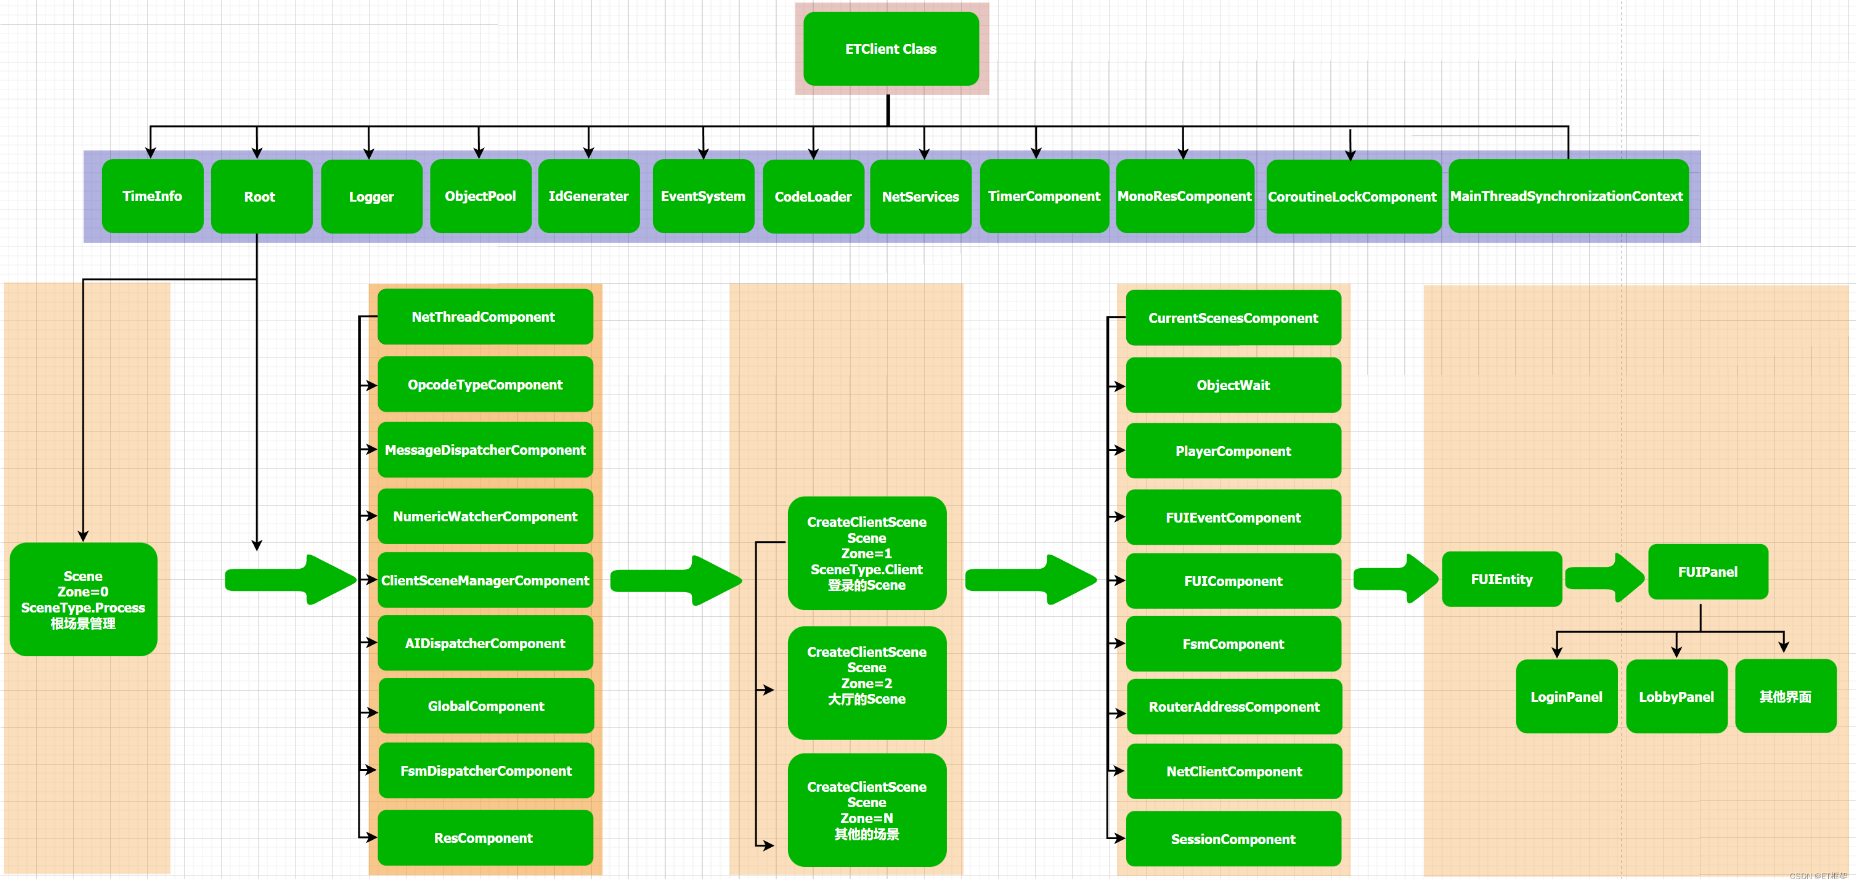
\includegraphics[width=.9\linewidth]{./pic/ET_20230512_143227.png}

\subsection{ET6 Beta(master) 设计的几点儿思路【帮助自己理解和梳理框架】【爱表哥,爱生活!!!任何时候,亲爱的表哥的活宝妹就是一定要、一定会嫁给活宝妹的亲爱的表哥!!!爱表哥,爱生活!!!】}
\label{sec-11-1}
\begin{itemize}
\item 之前每个功能是一个进程,比如realm gate location map,现在改成每个功能是一个Scene,一个Scene可以放到一个进程中。这样一台物理机先启动固定的进程,然后各个scene放到进程中运行。非常类似docker。【这个地方,有个早在ET6 时就如此重构的初衷,要看明白】
\begin{itemize}
\item 小伙伴问: et一开始就是多进程嘛…没毛病.不过现在是在进程内又开辟了相对独立的容器.熊猫能说说这么改的实际应用场景吗…什么实际需求促使了你做这个大刀阔斧的改动
\item 原因是【很多动态副本跟分线的需求】,现在可以16核机器起16个进程,然后【动态分配副本跟分线到进程上】(这里是说,必须重构为每个功能是一个Scene,一个Scene可以放到一个进程中之后,才可以实现,【动态分配副本跟分线到进程上】!而重构之前,就是动态副本到了每台物理机的多进程上,性能上会是极大的浪费)。比如很多单人副本,没必要一下子开很多进程来支持。(重构后,可以实现)需要的时候找一个负载低的进程动态创建一个(是动态创建一个到了一个核一个已经有任务在身的低消耗的在用进程上,而不需要再占用一台物理机N 多核与N 多进程,或弄新进程。也就是说,最大限度地发挥了每台物理机、每个核每个进程的性能表现)就行了,用完就可以回收了。
\end{itemize}
\item 所有的Scene放在一个进程就变成了AllServer模式。(【所以,自己没能体会透彻的时候,手动再添加一个什么 AllServer 是不对的。。】)
\item 服务器内部全部使用actor发送消息,比如realm发给gate,其实是发个actor消息到gate scene( 【这个,大概是Actor 消息的帮助类里,需要手动序列化,手动添加发送消息与返回消息的 actorId 的原因,内网消息手动序列化。。】)
\item dbserver将取消,每个进程直连mongodb,使用异步调用存取数据(这是,自己还没能想透的【区】的概念,一个小区里,有哪些小服?)
\item 协程锁简化了很多实现,例如location队列,actor队列,mailbox消息队列,全部使用协程锁实现,代码非常精简。(没理解透)
\item Scene可以开服前配置好在哪个进程(比如realm gate)也可以动态创建(比如副本,分线场景)。动态创建Scene回收Scene非常简单。
\end{itemize}
\subsection{Domain: 这个东西,不知道它是什么}
\label{sec-11-2}
\begin{itemize}
\item domain就是指这个entity属于哪个scene,毕竟一个进程上可以容纳多个scene
\item domain还有个很重要的作用,就是设置domain的时候才会执行反序列化system,还有注册eventsystem. 【这个看不懂,不知道它在说什么】
\item domain简单说是指属于哪个scene, 每个entity都有个domain字段,这样写逻辑方便能拿到自己scene上的数据
\end{itemize}
\subsection{AppType ==》 SceneType 重构}
\label{sec-11-3}
\begin{itemize}
\item 多进程多scene,具体scene放到那个进程完全取决于配制,全放到一个进程就是allserver了
\item 如果是个很大的scene,需要容纳很多人,可能就需要单独占用一个进程,这样才能完全利用一个核
\item 把每个scene都分配一个进程,就跟5.0差不多了
\end{itemize}


\section{IMHandler 接口实现的各种类型消息处理器:需要先理解透彻ETTask 和 ETVoid:}
\label{sec-12}
\begin{itemize}
\item 这个模块感觉还没有总结完。但因为还有111 个编译错误,很多我还不知道算是怎么回事。这个版块的总结放在后面,再改错误的时候带着问题来看更有效率。
\item 可以回去参考前一个游戏参考过的ET-EUI 里有一部分ETVoid 的相关使用,可以用作自己理解 ETTask ETVoid 的源码参考。ET-EUI 现笔记本里没有,可以拉一个下来。
\begin{itemize}
\item 【抓下来后用法基本一样,ETVoid 使用的地方基本一样】。不一样的地方是,它扩展(或者说 \textbf{重新自定义了} )了不少 \textbf{消息处理器接口类} 。那么就是说,ET-EUI 并没有、也做不到一个框架整个框架只使用一个消息处理器接口
\end{itemize}
\item 【主要使用:】主要是【服务端】处理客户端消息请求,用来定义处理逻辑。但是网络调用与返回大多是异步的,所以会有很多使用 ETTask 或是 ETVoid|Void 作为返回值的地方。主要是两个常用方法的接口定义,兼顾整个框架的接口定义。
\item \textbf{【参照ET-EUI】} :如果再来参照这个例子项目,或许也可以多定义几个不同的消息处理器接口,就不必强制整个框架只实现一个接口而顾A 顾不了B 了。那么如果下午继续参照这个例子,头脑清醒的时候,就要搞明白: \textbf{不同接口类,到底适用哪类消息?【可以把这部分再分析理解一下,总结在下面,但是区分清楚,哪个来自ET-EUI】} 就是需要理解透彻再改,不要再循环无限制地改。
\item 【两点不透彻:】ETTask|ETVoid|Void 到底使用什么返回值?另则, async-await 方法是定义为异步,还是非异步。如果 async 定义异步,什么地方必须有 await 调用?
\item 感觉ETTask|ETVoid 基本弄明白了,可是这里仍然是整个框架,感觉最为复杂不好修改的地方。可能我还是把网络异步调用没能弄得狠明白。
\begin{itemize}
\item 要保证两个方法里,若是同步方法, 方法中就一定不能有需要异步等待的地方(否则运行时会抛异常,对象为空之类的各种因为异步操作不能及时完成而抛的空异常)。就是, \textbf{如果需要使用异步方法,不可以改为同步,同步返回 void 或其它任何.}
\item 改的过程中,方法中曾经有过 await 调用异步方法的逻辑(方法),不能因想去掉编译错误就去掉 await 调用关键字,错误地改成同步方法,因为暂时去掉了编译错误,运行时一定会抛异常。
\item 【爱表哥,爱生活!!!任何时候,亲爱的表哥的活宝妹,就是一定要嫁给亲爱的表哥!!!爱表哥,爱生活!!!】
\end{itemize}
\end{itemize}
\subsection{IMHandler: interface 消息处理器接口类。它有2 个实现抽象类:AMHandler,AMRpcHandler}
\label{sec-12-1}
\begin{itemize}
\item 实现这个接口类型主要分为两个抽象类:AMHandler,AMRpcHandler. 所以ET 框架里现有一个接口IMHandler, 两个抽象实现类。其它是参考自ET-EUI.
\item 今天上午暂时只看取了这个接口,和两个抽象方法这里。后面任何的个体实现类,都还没有细看,不太懂。
\end{itemize}
\begin{minted}[fontsize=\scriptsize,linenos=false]{csharp}
public interface IMHandler {
    // 下面,返回类型不对:【暂时不作重点】
    void Handle(Session session, object message); // 这里返回类型,仍然应该是ETTask, 或者可能的 ETVoid ?

    // 消息处理器帮助类,在程序域加载的时候,会自动扫描程序域里的ActorMessageHander 标签,
    // 会想要拿消息的【发送类型】与消息的【返回类型】,来系统化管理消息处理
    // 所以,这里关于往返消息类型的API, 一个也不能少
    Type GetMessageType();
    Type GetResponseType(); // 不应该把这个去掉。
}
\end{minted}
\subsection{AMHandler<Message>: abstract 抽象基类:两个方法的返回类型,成为现在全框架的理解与实现难点}
\label{sec-12-2}
\begin{itemize}
\item AMHandler类,这个类相比AMRpcHandler更加简单一些,因为这个类型的处理,不需要关心回消息
\item 实现了接口IMHandler的Handle异步方法,具体逻辑为:
\begin{itemize}
\item 将传进来的msg首先转换为模板类,在AMHandler类里面为Message,具体应该为实现AMHandler的类的具体数据类。
\item 根据数据类,以及session生成一些报错日志,方便调试
\item 调用Run方法,将session及具体的数据类传进去
\item 实际继承抽象类AMHandler的类型,会实现这个接口,从而走向各自的处理。
\begin{minted}[fontsize=\scriptsize,linenos=false]{csharp}
public abstract class AMHandler<Message>: IMHandler where Message : class {

    protected abstract ETTask Run(Session session, Message message); // ET7 原本的
// 虽然我这么改,可以暂时消掉编译错误。但改得不对,现在消掉了编译错误,等编译通过,运行时错误会一再崩出来的。。。
    // protected abstract void Run(Session session, Message message); 

    public void Handle(Session session, object msg) {
        Message message = msg as Message;
        if (message == null) {
            Log.Error($"消息类型转换错误: {msg.GetType().Name} to {typeof (Message).Name}");
            return;
        }
        if (session.IsDisposed) {
            Log.Error($"session disconnect {msg}");
            return;
        }
        this.Run(session, message).Coroutine(); // 同步方法:调用的是异步方法的协程?可以这么写吗》?
    }
    public Type GetMessageType() {
        return typeof (Message);
    }
    public Type GetResponseType() {
        return null;
    }
}
\end{minted}
\end{itemize}
\end{itemize}
\subsection{AMRpcHandler: 去抓的ET7 框架的源码,可以用来【校正】其它被自己改错的}
\label{sec-12-3}
\begin{itemize}
\item 注意,在ET7 框架里,IMHandler 接口,与AMHandler 是定义在Share 双端共用。而AMRpcHandler 是定义在服务器端的,只有服务端存在进程间通信 Rpc 消息?
\item 去抓的ET7 框架的源码,可以用来校正其它被自己改错的类,或是方法定义。
\item 这个类比AMHandler要多传入一个模板类,主要用于处理那些约定好带返回数据的。 \textbf{【注意下面,是参考网络上别人的理解】} 。他们同样与活宝妹一样,也是一知半解,狠多地方说得也未必对。
\item 简单解释一下,现在ET协议数据主要分为两个类型,一种是来了消息直接自己处理的,另外一种是来了消息,自己处理完毕后,还需要将一些数据给返回的。【带返回类型,和不带返回类型】的消息。觉得它理解得不对,不适用于这里。因为 Rpc 这里感觉,更多的是说,进程间,或是现在ET7 重构后的不同SceneType 之间,比如注册登录服与网关服间的消息,内网消息等? Rpc-rpc-rpc\ldots{}
\item 主要的处理流程与AMHandler大体相同,需要注意的:
\begin{itemize}
\item 传入的模板类有类型要求,除了是class外,第一个需要是实现IRequest接口,第二个是实现IResponse接口,他们分别对应了传进来的协议数据类型,以及需要返回的协议数据类型。
\item IRequest类型,具有RpcId,这个id用来标识一个传入协议数据,同时又将它设置到response返回数据中的RpcId中,这样发送数据返回的时候,就能找到那个和他具有相同RpcId传入协议数据,这种关系一对一,从而能进行进一步处理。 \textbf{【谁发来的消息,就返回消息给谁——发送者】}
\item \uline{回调函数Reply(),即当处理完传入数据后,需要马上装配好返回数据,并将其发送回去,所以需要一个回调函数将response,通过session发送回去.} 前面说的是以前的框架。现在的回调过程,直接通过Session 会话框走网络层将消息发回去,不用再弄个Action<T> 来触发调用回调了。
\item 在Run中,需要传输上下文session,接受的协议数据request,需要返回的协议数据response,以及回调函数reply
\end{itemize}
\item 亲爱的表哥,活宝妹的小鼠标到了,可是活宝妹的小小手,也感觉这个好小,捏不住,不好用!!!
\end{itemize}
\begin{minted}[fontsize=\scriptsize,linenos=false]{csharp}
public abstract class AMRpcHandler<Request, Response>: IMHandler where Request : class, IRequest where Response : class, IResponse {
// ET7 框架里原本的:
    protected abstract ETTask Run(Session session, Request request, Response response);
    public void Handle(Session session, object message) { 
        HandleAsync(session, message).Coroutine();
    }
    private async ETTask HandleAsync(Session session, object message) {
        try {
            Request request = message as Request;
            if (request == null) 
                throw new Exception($"消息类型转换错误: {message.GetType().Name} to {typeof (Request).Name}");
            int rpcId = request.RpcId;
            long instanceId = session.InstanceId;
            Response response = Activator.CreateInstance<Response>(); // 创建一个消息的回复实例
            try { // 【找个例子看一下,例子在下面】不懂:下面一句是在干什么,执行对发送来消息的处理,写返回数据?这里调的是抽象异步函数。会在具体的实现类里去实现
// 猜测:应该更多可能是,通过不同服的具体实现,将返回数据写好?【是这样的】因为发送还在后面 session.Send(response) 是发送出去
                await this.Run(session, request, response); 
            }
            catch (Exception exception) { // 如果出异常:写异常结果
                Log.Error(exception);
                response.Error = ErrorCore.ERR_RpcFail;
                response.Message = exception.ToString();
            }
            // 等回调回来,session可以已经断开了,所以需要判断session InstanceId是否一样
            if (session.InstanceId != instanceId) 
                return;
            response.RpcId = rpcId; // 在这里设置rpcId是为了防止在Run中不小心修改rpcId字段。【谁发来的消息,就返回消息给谁——发送者】
            session.Send(response); // 把返回消息发回去,这里才是真正的发返回消息回请求端
        }
        catch (Exception e) { // 捕获异步操作过程中的异常
            throw new Exception($"解释消息失败: {message.GetType().FullName}", e);
        }
    }

    public Type GetMessageType() {
        return typeof (Request);
    }
    public Type GetResponseType() {
        return typeof (Response);
    }
}
\end{minted}
\subsection{C2R\_LoginHandler: AMRpcHandler 的一个实体类,前后版本封装对比}
\label{sec-12-4}
\begin{itemize}
\item 上面的 AMRpcHandler 抽象方法 Run() 不是看不懂吗,找到一个例子,有前后两个版本的对比,可以参看理解一下
\item 感觉今天下午,终于可以把先前这个自己总感觉迷迷糊糊的各种服的消息处理弄明白了
\item 今天下午,把所有这类各种服的消息处理里的这些问题、编译错误全部改掉。【爱表哥,爱生活!!!任何时候,活宝妹就是一定要嫁给亲爱的表哥!!!】
\end{itemize}
\begin{minted}[fontsize=\scriptsize,linenos=false]{csharp}
// 框架中原本有这个方法,为什么我需要把它改成下现在的这个样子?
[MessageHandler(SceneType.Realm)]
public class C2R_LoginHandler : AMRpcHandler<C2R_Login, R2C_Login> {
    // 【ET7 的进一步精简封装】:封装在AMRpcHandler 抽象实现类里
    protected override async ETTask Run(Session session, C2R_Login request, R2C_Login response) {
        // 随机分配一个Gate
        StartSceneConfig config = RealmGateAddressHelper.GetGate(session.DomainZone());
        Log.Debug($"gate address: {MongoHelper.ToJson(config)}");
			
        // 向gate请求一个key,客户端可以拿着这个key连接gate
        G2R_GetLoginKey g2RGetLoginKey = (G2R_GetLoginKey) await ActorMessageSenderComponent.Instance.Call(
            config.InstanceId, new R2G_GetLoginKey() {Account = request.Account});

        response.Address = config.InnerIPOutPort.ToString();
        response.Key = g2RGetLoginKey.Key;
        response.GateId = g2RGetLoginKey.GateId;
    }

    // 【ET-EUI 版本中的实现】:用来作ET7 重构的对比参照。【下面的方法不要,不再需要】
    protected override async void Run(Session session, C2R_Login message, Action<R2C_Login> reply) { // 【古老封装:】自己看看就能弄明白,ET7 的进一步精简封装
        R2C_Login response = new R2C_Login(); // 创建一个回复消息的实例:是因为没有实例,参数只有回调方法函数,所以必须得造一个。。
        try {
            // if (message.Account != "abcdef" || message.Password != "111111") // 这里作必要的错误检测
            // {
            //    response.Error = ErrorCode.ERR_AccountOrPasswordError;
            //    reply(response);
            //    return;
            // }
            // 随机分配一个Gate: 这里原理不变
            StartSceneConfig config = RealmGateAddressHelper.GetGate(session.DomainZone());
            Log.Debug($"gate address: {MongoHelper.ToJson(config)}");
            // 向gate请求一个key,客户端可以拿着这个key连接gate
            G2R_GetLoginKey g2RGetLoginKey = (G2R_GetLoginKey) await ActorMessageSenderComponent.Instance.Call(
                config.InstanceId, new R2G_GetLoginKey() {Account = message.Account});
            // 手动:写返回消息的内容
            response.Address = config.InnerIPOutPort.ToString();
            response.Key = g2RGetLoginKey.Key;
            response.GateId = g2RGetLoginKey.GateId;
            reply(response); // 通过调用回调函数,将回调回调到调用端,就是把写好的消息返回给调用端,供它拿数据接通知等
        }
        catch (Exception e) { // 网络异步的过程中,捕获异常
            ReplyError(response, e, reply);
        }
    }
}
\end{minted}

\subsection{IMHandler 【ET-EUI】:主要是与上面对比}
\label{sec-12-5}
\begin{itemize}
\item 因为对于ET-EUI 里,它为什么要再多自定义几个接口,这个版块不够熟悉
\item 我觉得把两个框架的几个接口与抽象实体类提出来对比理解一下是对的,因为没明白,为什么ET7 里会重构成那个样子。可能也网上查下再帮助理解一下。
\end{itemize}
\begin{minted}[fontsize=\scriptsize,linenos=false]{csharp}
public interface IMHandler {
    void Handle(Session session, object message);
    Type GetMessageType();
    Type GetResponseType();
    // ETTask Run(Session session, M2C_TestActorMessage message); // 把这里去掉,感觉加得不对
}
\end{minted}
\subsection{IMActorHandler: 【ET-EUI:仅作参考】大概参考 ET-EUI 来的,它的目的应该是把最基类的接口,与其它两类的接口相区分开来}
\label{sec-12-6}
\begin{itemize}
\item 从这个小节开始,主要是整理的ET-EUI 里面的接口与抽象实现类。可能主要两个实现扩展类:(A|I)MHandler, (A|I)MRpcHandler, 都看一下
\item 大概参考 ET-EUI 来的,它的目的应该是把最基类的接口,与其它两类的接口相区分开来。但是,我想、猜测、理解的话,应该是上面一个接口,如果能够把ETTask 与ETVoid 狠好地统一的话,应该一个接口可能可以足以整个框架使用的。
\item 消息处理器:基本可以理解为,总都是【服务端】的消息处理器。【客户端】更多的是发请求消息,和接收消息。客户端狠少涉及什么消息处理。
\item 下面的接口,哪个例子也没有参照,自己改的。极有可能都是错的
\end{itemize}
\begin{minted}[fontsize=\scriptsize,linenos=false]{csharp}
public interface IMActorHandler {
    // 下面,参考的是ET-EUI 可能是 6.0 版本。ET7 里,可能接口还可以简化,还是Actor 消息机制模块简化了,不一定如下面这样
    void Handle(Entity entity, int fromProcess, object actorMessage);
    // ETTask Handle(Entity entity, object actorMessage, Action<IActorResponse> reply);
    Type GetRequestType();
    Type GetResponseType();
}
\end{minted}
\subsection{AMActorLocationHandler: 源码被我改动了}
\label{sec-12-7}
\begin{itemize}
\item 源码被我改动了,正确性与否没有关系,主要是帮助自己梳理一下几大不同的类型,到改编译错误的时候,能够边修改边弄明白。
\begin{minted}[fontsize=\scriptsize,linenos=false]{csharp}
[EnableClass]
public abstract class AMActorLocationHandler<E, Message>: IMActorHandler where E : Entity where Message : class, IActorLocationMessage {
    // protected abstract ETTask Run(E entity, Message message);
    protected abstract void Run(E entity, Message message);
    // public async ETTask Handle(Entity entity, int fromProcess, object actorMessage) {
    public void Handle(Entity entity, int fromProcess, object actorMessage) {
        if (actorMessage is not Message message) {
            Log.Error($"消息类型转换错误: {actorMessage.GetType().FullName} to {typeof (Message).Name}");
            return;
        }
        if (entity is not E e) {
            Log.Error($"Actor类型转换错误: {entity.GetType().Name} to {typeof (E).Name} --{typeof (Message).Name}");
            return;
        }
        ActorResponse response = new() {RpcId = message.RpcId};
        ActorHandleHelper.Reply(fromProcess, response);
        // await this.Run(e, message);
        this.Run(e, message);
    }
    public Type GetRequestType() {
        return typeof (Message);
    }
    public Type GetResponseType() {
        return typeof (ActorResponse);
    }
}
\end{minted}
\end{itemize}
\subsection{AMActorLocationRpcHandler: 上面接口实现类的一个使用例子。我把返回参数改了}
\label{sec-12-8}
\begin{minted}[fontsize=\scriptsize,linenos=false]{csharp}
[EnableClass]
public abstract class AMActorLocationRpcHandler<E, Request, Response>: IMActorHandler where E : Entity where Request : class, IActorLocationRequest where Response : class, IActorLocationResponse {
    // protected abstract ETTask Run(E unit, Request request, Response response);
    protected abstract void Run(E unit, Request request, Response response);
    // public async ETTask Handle(Entity entity, int fromProcess, object actorMessage) {
    public void Handle(Entity entity, int fromProcess, object actorMessage) {
        try {
            if (actorMessage is not Request request) {
                Log.Error($"消息类型转换错误: {actorMessage.GetType().FullName} to {typeof (Request).Name}");
                return;
            }
            if (entity is not E ee) {
                Log.Error($"Actor类型转换错误: {entity.GetType().Name} to {typeof (E).Name} --{typeof (Request).Name}");
                return;
            }
            int rpcId = request.RpcId;
            Response response = Activator.CreateInstance<Response>();
            try {
                //await this.Run(ee, request, response);
                this.Run(ee, request, response);
            }
            catch (Exception exception) {
                Log.Error(exception);
                response.Error = ErrorCore.ERR_RpcFail;
                response.Message = exception.ToString();
            }
            response.RpcId = rpcId;
            ActorHandleHelper.Reply(fromProcess, response);
        }
        catch (Exception e) {
            throw new Exception($"解释消息失败: {actorMessage.GetType().FullName}", e);
        }
    }
    public Type GetRequestType() {
        return typeof (Request);
    }
    public Type GetResponseType() {
        return typeof (Response);
    }
    // 这里涉及的就是那个接口方法的定义
    public ETTask Handle(Entity entity, object actorMessage, Action<IActorResponse> reply) => throw new NotImplementedException();
}
\end{minted}
\subsection{AMActorLocationRpcHandler: Rpc 就是进程间消息(或是ET7 重构为SceneType 之后的多核间消息)}
\label{sec-12-9}
\begin{minted}[fontsize=\scriptsize,linenos=false]{csharp}
[EnableClass]
public abstract class AMActorLocationRpcHandler<E, Request, Response>: IMActorHandler where E : Entity where Request : class, IActorLocationRequest where Response : class, IActorLocationResponse {
    // protected abstract ETTask Run(E unit, Request request, Response response);
    protected abstract void Run(E unit, Request request, Response response);
    // public async ETTask Handle(Entity entity, int fromProcess, object actorMessage) {
    public void Handle(Entity entity, int fromProcess, object actorMessage) {
        try {
            if (actorMessage is not Request request) {
                Log.Error($"消息类型转换错误: {actorMessage.GetType().FullName} to {typeof (Request).Name}");
                return;
            }
            if (entity is not E ee) {
                Log.Error($"Actor类型转换错误: {entity.GetType().Name} to {typeof (E).Name} --{typeof (Request).Name}");
                return;
            }
            int rpcId = request.RpcId;
            Response response = Activator.CreateInstance<Response>();
            try {
                //await this.Run(ee, request, response);
                this.Run(ee, request, response);
            }
            catch (Exception exception) {
                Log.Error(exception);
                response.Error = ErrorCore.ERR_RpcFail;
                response.Message = exception.ToString();
            }
            response.RpcId = rpcId;
            ActorHandleHelper.Reply(fromProcess, response);
        }
        catch (Exception e) {
            throw new Exception($"解释消息失败: {actorMessage.GetType().FullName}", e);
        }
    }
    public Type GetRequestType() {
        return typeof (Request);
    }
    public Type GetResponseType() {
        return typeof (Response);
    }
}
\end{minted}
\subsection{ActorHandleHelper 静态帮助类:包装了必要的方法,帮助自动化回复相关回调消息 et3}
\label{sec-12-10}
\begin{itemize}
\item 再后面的,MessageDispatcherComponent 相关的,因为网络部分的再次总结一遍,移过去,先系统总结一下。改天有必要的时候,再作修改。
\end{itemize}


\section{ResourcesComponent 资源包管理器相关:有时候,拖拉机游戏里会需要拿它来加载图片}
\label{sec-13}
\subsection{ResourcesComponent: 同文件有其生成系}
\label{sec-13-1}
\begin{minted}[fontsize=\scriptsize,linenos=false]{csharp}
[ComponentOf]
public class ResourcesComponent: Entity, IAwake, IDestroy {
    public static ResourcesComponent Instance { get; set; }
    public AssetBundleManifest AssetBundleManifestObject { get; set; }
    public Dictionary<int, string> IntToStringDict = new Dictionary<int, string>();
    public Dictionary<string, string> StringToABDict = new Dictionary<string, string>();
    public Dictionary<string, string> BundleNameToLowerDict = new Dictionary<string, string>() { { "StreamingAssets", "StreamingAssets" } };
    public readonly Dictionary<string, Dictionary<string, UnityEngine.Object>> resourceCache =
        new Dictionary<string, Dictionary<string, UnityEngine.Object>>();
    public readonly Dictionary<string, ABInfo> bundles = new Dictionary<string, ABInfo>();
    // 缓存包依赖,不用每次计算
    public readonly Dictionary<string, string[]> DependenciesCache = new Dictionary<string, string[]>();
}
\end{minted}
\subsection{客户端 ConfigLoader 的Invoke 标签下:在根控件 Root 下添加资源管理器组件}
\label{sec-13-2}
\begin{minted}[fontsize=\scriptsize,linenos=false]{csharp}
[Invoke]
public class GetAllConfigBytes: AInvokeHandler<ConfigComponent.GetAllConfigBytes, Dictionary<Type, byte[]>> {
    public override Dictionary<Type, byte[]> Handle(ConfigComponent.GetAllConfigBytes args) {
        Dictionary<Type, byte[]> output = new Dictionary<Type, byte[]>();
        HashSet<Type> configTypes = EventSystem.Instance.GetTypes(typeof (ConfigAttribute));

        if (Define.IsEditor) {
            string ct = "cs";
            GlobalConfig globalConfig = Resources.Load<GlobalConfig>("GlobalConfig");
            CodeMode codeMode = globalConfig.CodeMode;
            switch (codeMode) {
            case CodeMode.Client:
                ct = "c";
                break;
            case CodeMode.Server:
                ct = "s";
                break;
            case CodeMode.ClientServer:
                ct = "cs";
                break;
            default:
                throw new ArgumentOutOfRangeException();
            }
            List<string> startConfigs = new List<string>() {
                "StartMachineConfigCategory", 
                "StartProcessConfigCategory", 
                "StartSceneConfigCategory", 
                "StartZoneConfigCategory",
            };
            foreach (Type configType in configTypes) {
                string configFilePath;
                if (startConfigs.Contains(configType.Name)) {
                    configFilePath = $"../Config/Excel/{ct}/{Options.Instance.StartConfig}/{configType.Name}.bytes";    
                }
                else {
                    configFilePath = $"../Config/Excel/{ct}/{configType.Name}.bytes";
                }
                output[configType] = File.ReadAllBytes(configFilePath);
            }
        } else {
            using (Root.Instance.Scene.AddComponent<ResourcesComponent>()) { // <<<<<<<<<<<<<<<<<<<< 
                const string configBundleName = "config.unity3d";
                ResourcesComponent.Instance.LoadBundle(configBundleName);

                foreach (Type configType in configTypes) {
                    TextAsset v = ResourcesComponent.Instance.GetAsset(configBundleName, configType.Name) as TextAsset;
                    output[configType] = v.bytes;
                }
            }
        }
        return output;
    }
}
\end{minted}


\section{Coroutine 锁之类的相关总结:【任何时候,亲爱的表哥的活宝妹就是一定要嫁给亲爱的表哥!!!爱表哥,爱生活!!!】}
\label{sec-14}
\begin{itemize}
\item 这个模块,现在再看,这里、这个章节里,被总结得乱七八糟。但现在因为真正读懂看懂,暂时不更改更新这个模块,继续去看其它自己不曾弄懂的。等31 号搬进新住处后,会把重构游戏编译错误继续改完、重构好。【爱表哥,爱生活!!!任何时候,亲爱的表哥的活宝妹就是一定要、一定会嫁给活宝妹的亲爱的表哥!!!爱表哥,爱生活!!!】
\item 【锁的两套机制:】主要是【创建】与【回收】。
\item \textbf{【CoroutineLockComponent单例组件】} 模块用到,两种类型的锁:【异步共享资源异步等待锁】+【共享资源独占锁】
\item 【异步共享资源异步等待锁】:框架里,帮助实现,对异步共享资源的,自动挂号排队站队,作为中介帮助调用方拿到可以持有共享资源的【独占锁】
\item 【共享资源独占锁】:最基本的,实现对多进程、多线程?共享资源的安全保护,尤其是写数据安全保护
\item 【协程锁组件】单例类,Update() 更新回调实现
\item 重构后的模块,是单例类管理组件,不同于框架里其它组件,热更域里自带生成系或说更新系。它是单例,是定义死了的。【任何时候,亲爱的表哥的活宝妹就是一定要嫁给亲爱的表哥!!爱表哥,爱生活!!!活宝妹还没能嫁给亲爱的表哥,就时间停止,世界不转,直到活宝妹可以嫁给亲爱的表哥的这一天!!】
\end{itemize}
\subsection{CoroutineLockType: 静态类定义的几种类型}
\label{sec-14-1}
\begin{itemize}
\item 【爱表哥,爱生活!!!任何时候,亲爱的表哥的活宝妹就是一定要、一定会嫁给活宝妹的亲爱的表哥!!!爱表哥,爱生活!!!】
\item 【爱表哥,爱生活!!!任何时候,亲爱的表哥的活宝妹就是一定要、一定会嫁给活宝妹的亲爱的表哥!!!爱表哥,爱生活!!!】
\item 【爱表哥,爱生活!!!任何时候,亲爱的表哥的活宝妹就是一定要、一定会嫁给活宝妹的亲爱的表哥!!!爱表哥,爱生活!!!】
\item 【爱表哥,爱生活!!!任何时候,亲爱的表哥的活宝妹就是一定要、一定会嫁给活宝妹的亲爱的表哥!!!爱表哥,爱生活!!!】
\item 【爱表哥,爱生活!!!任何时候,亲爱的表哥的活宝妹就是一定要、一定会嫁给活宝妹的亲爱的表哥!!!爱表哥,爱生活!!!】
\item 【爱表哥,爱生活!!!任何时候,亲爱的表哥的活宝妹就是一定要、一定会嫁给活宝妹的亲爱的表哥!!!爱表哥,爱生活!!!】
\item 【爱表哥,爱生活!!!任何时候,亲爱的表哥的活宝妹就是一定要、一定会嫁给活宝妹的亲爱的表哥!!!爱表哥,爱生活!!!】
\item 【爱表哥,爱生活!!!任何时候,亲爱的表哥的活宝妹就是一定要、一定会嫁给活宝妹的亲爱的表哥!!!爱表哥,爱生活!!!】
\item 【爱表哥,爱生活!!!任何时候,亲爱的表哥的活宝妹就是一定要、一定会嫁给活宝妹的亲爱的表哥!!!爱表哥,爱生活!!!】
\item 【爱表哥,爱生活!!!任何时候,亲爱的表哥的活宝妹就是一定要、一定会嫁给活宝妹的亲爱的表哥!!!爱表哥,爱生活!!!】
\item 就是定义框架中用到的几种使用协程锁的情境,分成几种不同的类型
\end{itemize}
\begin{minted}[fontsize=\scriptsize,linenos=false]{csharp}
// 【下面,各种强调】:不用协程锁的使用上下文场景的类型,这个【使用上下文场景类型】,定义的究竟是什么,不同类型之间,是如何区分的?
// 分别对应以下使用情景:
    // 多个向location查询同一个实体真实进程号地址(在访问跨进程实体时)【这里是,位置服中的被查询的实体的相关信息, 会被锁,被查询者!】,访问一次获得进程地址即可 ;
    // 【多个针对同一个实体对象,发起的Actor消息】;这里是【发送Actor 消息的实体】,同一个实体,发送消息是并发,一次只能发一个消息。加锁是因为,单线程多进程框架里,多个进程想要消息入队这个可【发送消息的 actorid】,对ActorLocationSender 队列上锁?
    // 多个处理针对同一个实体的Mailbox消息处理,处理需要按照先后顺序;
    // 针对Map中单位上下线时,新上线消息需要等待下线消息执行完后再处理;(自己先前接触过的,玩家客户端某端下线、某端上线、或自顶号操作,保证执行先后顺序的锁,锁住针对的是,一个某定玩家 UnitId)
    // 针对同一个DB访问的前后顺序处理;
    // 多个资源请求同一个ab包下载的处理。
// 【可添加自定义类型:】如果还有自己想要处理的协程锁类型,可自行添加,不过现在这些应该已经够用了,且ET6.0中猫大大部分都已经封装处理好了,不需要我们再写了。
public static class CoroutineLockType { // 对应的,就是框架里,线程安全、资源安全,几处使用到锁的上下文场景
    public const int None = 0;
    public const int Location = 1;                  // location 场景上使用,不是什么进程,重构了
    public const int ActorLocationSender = 2;       // ActorLocationSender中队列消息。【重点看这个】: 这个【A发请求拿B 位置的消息】,发起者A, 与【被请求者B】, 锁的是发问者A
    public const int Mailbox = 3;                   // Mailbox中队列
    public const int UnitId = 4;                    // Map服务器上线下线时使用
    public const int DB = 5;
    public const int Resources = 6;
    public const int ResourcesLoader = 7;
    public const int Max = 100; // 这个必须最大
}
\end{minted}
\subsection{CoroutineLock: 里面的 level 参数,不懂}
\label{sec-14-2}
\begin{minted}[fontsize=\scriptsize,linenos=false]{csharp}
public class CoroutineLock: IDisposable { // 【协程锁】: level 是什么意思呢?
    private int type;
    private long key;
    private int level;
    public static CoroutineLock Create(int type, long k, int count) {
        CoroutineLock coroutineLock = ObjectPool.Instance.Fetch<CoroutineLock>(); // 对象池管理,回收再利用等
        coroutineLock.type = type;
        coroutineLock.key = k;
        coroutineLock.level = count;
        return coroutineLock;
    }
    public void Dispose() {
        CoroutineLockComponent.Instance.RunNextCoroutine(this.type, this.key, this.level + 1); // <<<<<<<<<<<<<<<<<<<< 跟进去
        this.type = CoroutineLockType.None;
        this.key = 0;
        this.level = 0;
        ObjectPool.Instance.Recycle(this);
    }
}
\end{minted}
\subsection{WaitCoroutineLock: 【等待协程锁】:为什么它也要设置超时机制?}
\label{sec-14-3}
\begin{minted}[fontsize=\scriptsize,linenos=false]{csharp}
// 【协程超时、自动检测机制】:问题是,协程原本就每桢执行一次,为什么有必要设置【 1 (毫)秒?用得多就包装一下?】超时?
[Invoke(TimerCoreInvokeType.CoroutineTimeout)] // 自动检测超时机制:不知道为什么定义静态类 TimerCoreInvokeType ?
public class WaitCoroutineLockTimer: ATimer<WaitCoroutineLock> {
    protected override void Run(WaitCoroutineLock waitCoroutineLock) {
        if (waitCoroutineLock.IsDisposed()) return; // 若已回收,再无它
        waitCoroutineLock.SetException(new Exception("coroutine is timeout!")); // 抛超时异常
    }
}
public class WaitCoroutineLock {
    private ETTask<CoroutineLock> tcs; // 成员变量 
    public static WaitCoroutineLock Create() {
        WaitCoroutineLock waitCoroutineLock = new WaitCoroutineLock();
        waitCoroutineLock.tcs = ETTask<CoroutineLock>.Create(true); // <<<<<<<<<<<<<<<<<<<< 对象池中抓壮丁
        return waitCoroutineLock;
    }
    public void SetResult(CoroutineLock coroutineLock) {
        if (this.tcs == null) 
            throw new NullReferenceException("SetResult tcs is null");
        var t = this.tcs;
        this.tcs = null;
        t.SetResult(coroutineLock);
    }
    public void SetException(Exception exception) {
        if (this.tcs == null) 
            throw new NullReferenceException("SetException tcs is null");
        var t = this.tcs;
        this.tcs = null;
        t.SetException(exception);
    }
    public bool IsDisposed() {
        return this.tcs == null;
    }
    public async ETTask<CoroutineLock> Wait() {
        return await this.tcs;
    }
}
\end{minted}
\subsection{CoroutineLockQueue: 队列里面嵌套协程锁,没看懂}
\label{sec-14-4}
\begin{itemize}
\item 这里面有个以 WaitCoroutineLock 为元素的队列。还有一把当前锁。【不明白这个当前锁,要这个成员变量可以作什么?】
\item 当前锁为空时,直接创建返回一把新锁,不管时间什么的;当非空,创建新的等待锁,加入队列,赋值给当前锁,并返回。。
\item 队列,这里面的队列是做什么的?
\end{itemize}
\begin{minted}[fontsize=\scriptsize,linenos=false]{csharp}
public class CoroutineLockQueue { // 【协程锁队列】
    private int type; // 类型
    private long key; // ?
    public static CoroutineLockQueue Create(int type, long key) {
        CoroutineLockQueue coroutineLockQueue = ObjectPool.Instance.Fetch<CoroutineLockQueue>();
        coroutineLockQueue.type = type;
        coroutineLockQueue.key = key;
        return coroutineLockQueue;
    }
    private CoroutineLock currentCoroutineLock; // 当前锁
    private readonly Queue<WaitCoroutineLock> queue = new Queue<WaitCoroutineLock>(); // 【协程等待锁队列】
    public int Count {
        get {
            return this.queue.Count;
        }
    }
    public async ETTask<CoroutineLock> Wait(int time) { // 【这个方法】:没看懂,没理解,弄个协程等待锁,做什么有什么用?需要网上查下相关讲解
        // 从这里开始迷糊:两个不同的返回分支:
        if (this.currentCoroutineLock == null) {
            this.currentCoroutineLock = CoroutineLock.Create(type, key, 1); // level: 感觉,是纪录协程桢数序号,从 1 开始, 100-Warning
            return this.currentCoroutineLock; // 直接返回:返回一把锁,不管它时间怎么样的?。。。没懂
        }
        WaitCoroutineLock waitCoroutineLock = WaitCoroutineLock.Create(); // 创建等待锁
        this.queue.Enqueue(waitCoroutineLock); // 加入队列
        if (time > 0) { // 有等待时间:创建一个一次性闹钟。
            long tillTime = TimeHelper.ClientFrameTime() + time;
            // 重点去看:闹钟时间到,会做什么?【协程锁超时,自动检测回调到TimerCoreInvokeType.CoroutineTimeout 标记的类】超时后又只是回收掉。理解上逻辑连贯不起来
            // 等待的时间到了,等待协程锁异步任务会返回???
            TimerComponent.Instance.NewOnceTimer(tillTime, TimerCoreInvokeType.CoroutineTimeout, waitCoroutineLock);
        }
        this.currentCoroutineLock = await waitCoroutineLock.Wait();
        return this.currentCoroutineLock;
    }
    public void Notify(int level) { // 哪里会调用这个方法?只更新了 level 桢数或桢序号?
        // 有可能WaitCoroutineLock已经超时抛出异常,所以要找到一个未处理的WaitCoroutineLock
        while (this.queue.Count > 0) { // 遍历一遍队列:队列是,入队时间升序,超时时间没有、不曾排序的
            WaitCoroutineLock waitCoroutineLock = queue.Dequeue();
            if (waitCoroutineLock.IsDisposed()) continue; // 已经超时回收。这里,相当于从队列中将其清除
            CoroutineLock coroutineLock = CoroutineLock.Create(type, key, level);
            waitCoroutineLock.SetResult(coroutineLock); // 这些,狠嵌套。也狠欠扁,看不懂。。。
            break;
        }
    }
    public void Recycle() {
        this.queue.Clear();
        this.key = 0;
        this.type = 0;
        this.currentCoroutineLock = null;
        ObjectPool.Instance.Recycle(this);
    }
}
\end{minted}
\subsection{CoroutineLockQueueType: 【协程锁队列:分不同类型的】。字典管理一堆上面的 CoroutineLockQueue.}
\label{sec-14-5}
\begin{itemize}
\item 所以这个类极简单,字典的相关操作,就可以了。Notify() 调用相关相对应的CoroutineLockQueue 的相应方法就可以
\end{itemize}
\begin{minted}[fontsize=\scriptsize,linenos=false]{csharp}
public class CoroutineLockQueueType { // 叫个什么,类型。。。
    private readonly int type;
    private readonly Dictionary<long, CoroutineLockQueue> coroutineLockQueues = new Dictionary<long, CoroutineLockQueue>();
    public CoroutineLockQueueType(int type) {
        this.type = type;
    }
    private CoroutineLockQueue Get(long key) {
        this.coroutineLockQueues.TryGetValue(key, out CoroutineLockQueue queue);
        return queue;
    }
    private CoroutineLockQueue New(long key) {
        CoroutineLockQueue queue = CoroutineLockQueue.Create(this.type, key);
        this.coroutineLockQueues.Add(key, queue);
        return queue;
    }
    private void Remove(long key) {
        if (this.coroutineLockQueues.Remove(key, out CoroutineLockQueue queue)) 
            queue.Recycle();
    }
    public async ETTask<CoroutineLock> Wait(long key, int time) {
        CoroutineLockQueue queue = this.Get(key) ?? this.New(key);
        return await queue.Wait(time);
    }
    public void Notify(long key, int level) {
        CoroutineLockQueue queue = this.Get(key);
        if (queue == null) return;
        if (queue.Count == 0) this.Remove(key);
        queue.Notify(level); // <<<<<<<<<<<<<<<<<<<< 
    }
}
\end{minted}
\subsection{CoroutineLockComponent: 【单例组件】。源码读起来感觉简单,可是理解不透彻。那些等是等什么?}
\label{sec-14-6}
\begin{minted}[fontsize=\scriptsize,linenos=false]{csharp}
// 【协程锁组件】单例:Update() 更新回调实现
public class CoroutineLockComponent: Singleton<CoroutineLockComponent>, ISingletonUpdate { // Update() 生命周期函数调用 
    private readonly Dictionary<int, CoroutineLockQueueType> dictionary = new();
    private readonly Queue<(int, long, int)> nextFrameRun = new Queue<(int, long, int)>(); // 下一桢待更新的

    public override void Dispose() {
        this.nextFrameRun.Clear();
    }
    public void Update() { // 更新:每桢更新,一个个处理
        // 循环过程中会有对象继续加入队列
        while (this.nextFrameRun.Count > 0) {
            (int coroutineLockType, long key, int count) = this.nextFrameRun.Dequeue();
            this.Notify(coroutineLockType, key, count);
        }
    }
    public void RunNextCoroutine(int coroutineLockType, long key, int level) { // 【CoroutineLock】回收时也会调用,想想这个调用问题
        // 一个协程队列一帧处理超过100个,说明比较多了,打个warning,检查一下是否够正常
        if (level == 100) 
            Log.Warning($"too much coroutine level: {coroutineLockType} {key}");
        this.nextFrameRun.Enqueue((coroutineLockType, key, level)); // 加入到:下一桢待处理的队列中去
    }
    public async ETTask<CoroutineLock> Wait(int coroutineLockType, long key, int time = 60000) {
        CoroutineLockQueueType coroutineLockQueueType;
        if (!this.dictionary.TryGetValue(coroutineLockType, out coroutineLockQueueType)) {
            coroutineLockQueueType = new CoroutineLockQueueType(coroutineLockType);
            this.dictionary.Add(coroutineLockType, coroutineLockQueueType);
        }
        return await coroutineLockQueueType.Wait(key, time);
    }
    private void Notify(int coroutineLockType, long key, int level) {
        CoroutineLockQueueType coroutineLockQueueType;
        if (!this.dictionary.TryGetValue(coroutineLockType, out coroutineLockQueueType)) return;
        coroutineLockQueueType.Notify(key, level); // 【自顶向下】地调用,每桢更新时,自顶向下地更新
    }
}
\end{minted}
\begin{itemize}
\item 【任何时候,亲爱的表哥的活宝妹就是一定要嫁给亲爱的表哥!!爱表哥,爱生活!!!】
\item 【任何时候,亲爱的表哥的活宝妹就是一定要嫁给亲爱的表哥!!爱表哥,爱生活!!!】
\item 【任何时候,亲爱的表哥的活宝妹就是一定要嫁给亲爱的表哥!!爱表哥,爱生活!!!】
\item 【任何时候,亲爱的表哥的活宝妹就是一定要嫁给亲爱的表哥!!爱表哥,爱生活!!!】
\item 【任何时候,亲爱的表哥的活宝妹就是一定要嫁给亲爱的表哥!!爱表哥,爱生活!!!】
\item 【任何时候,亲爱的表哥的活宝妹就是一定要嫁给亲爱的表哥!!爱表哥,爱生活!!!】
\item 【任何时候,亲爱的表哥的活宝妹就是一定要嫁给亲爱的表哥!!爱表哥,爱生活!!!】
\item 【任何时候,亲爱的表哥的活宝妹就是一定要嫁给亲爱的表哥!!爱表哥,爱生活!!!】
\item 【任何时候,亲爱的表哥的活宝妹就是一定要嫁给亲爱的表哥!!爱表哥,爱生活!!!】
\item 【任何时候,亲爱的表哥的活宝妹就是一定要嫁给亲爱的表哥!!爱表哥,爱生活!!!】
\item 【任何时候,亲爱的表哥的活宝妹就是一定要嫁给亲爱的表哥!!爱表哥,爱生活!!!】
\item 【任何时候,亲爱的表哥的活宝妹就是一定要嫁给亲爱的表哥!!爱表哥,爱生活!!!】
\item 【任何时候,亲爱的表哥的活宝妹就是一定要嫁给亲爱的表哥!!爱表哥,爱生活!!!】
\item 【任何时候,亲爱的表哥的活宝妹就是一定要嫁给亲爱的表哥!!爱表哥,爱生活!!!】
\end{itemize}
% Emacs 28.2 (Org mode 8.2.7c)
\end{document}